\documentclass{article}

% Recommended MLSys packages
\usepackage{microtype}
\usepackage{graphicx}
\usepackage{subfigure}
\usepackage{booktabs}
\usepackage{amsmath,amssymb}
\usepackage{longtable,array,calc}
\usepackage{hyperref}
\newcommand{\theHalgorithm}{\arabic{algorithm}}
\newcommand{\degree}{\ensuremath{^\circ}}

% MLSys 2025 style
\usepackage{mlsys2025}
\mlsystitlerunning{Razor's Edge Dynamic Batching}
\providecommand{\tightlist}{\setlength{\itemsep}{0pt}\setlength{\parskip}{0pt}}

\begin{document}

\twocolumn[
\mlsystitle{Razor's Edge: Throughput Optimized Dynamic Batching with Latency Objectives}

\begin{mlsysauthorlist}
\mlsysauthor{Arrman Anicket Saha}{ind}
\end{mlsysauthorlist}
\mlsysaffiliation{ind}{Independent Researcher, USA}
\mlsyscorrespondingauthor{Arrman Anicket Saha}{arrmansa99@gmail.com}
\mlsyskeywords{Batching, Scheduling, Inference Serving, Throughput Optimization}

\vskip 0.3in
\begin{abstract}
Serving systems for embedding, LLM, and other
matrix-multiplication-dominated inference workloads rely on batching for
efficient hardware utilization. We observe that batching efficiency
exhibits a sharp input-size-dependent structure driven by the transition
between memory-bound and compute-bound regimes: small inputs can be
batched flexibly across heterogeneous sizes, while large inputs require
near-uniformity, leading to a rapid collapse in batching efficiency.
This produces a characteristic blade-like ("razor\textquotesingle s
edge") shape in the batch performance landscape.

We present the Razor\textquotesingle s Edge batching scheduler, a
practical framework that combines (i) dynamic-programming-based
throughput optimization over sorted requests, (ii) production-oriented
next-batch selection strategies (\texttt{FIFO}, \texttt{MINMAX}, and
\texttt{GUARDED\_BATCH\_SIZE}), and (iii) startup-time-efficient model
benchmarking that builds batch timing estimators from direct
measurements on the same hardware where the model is deployed. A central
novelty claim in this paper is this measurement-to-optimizer bridge:
instead of relying on analytic proxy cost models, we benchmark the
deployed model/hardware pair and feed those empirical timings directly
into the DP cost table used for scheduling decisions. We also introduce
a practical visualization method for quantifying batching efficiency
improvements when expanding the allowed maximum batch size from (N-1) to
(N), producing the characteristic "razor\textquotesingle s edge" contour
plots. The approach is designed for real-time online serving with
queueing. Our claims are scoped to "ahead-of-time variable-size batching
for encoder-style inference" evaluated in this paper, not to universal
superiority across all serving stacks. We demonstrate the
scheduler\textquotesingle s efficacy through a 47\% throughput increase
on a CPU embedding workload (\texttt{jina-embeddings-v2-base-en}), a
26\% throughput increase on a GPU embedding workload
(\texttt{BAAI/bge-m3}), and controllable latency/throughput trade-offs
across the final strategy set.

\end{abstract}

]

\printAffiliationsAndNotice{}
\hypertarget{1-introduction}{%
\section{Introduction}\label{1-introduction}}

Requests cannot be processed instantaneously at arrival in any real
serving system. Under load, queueing is inevitable. A first-come,
first-served single-request policy is simple, but it fails to exploit
throughput gains available through batching. Simply batching the first
\texttt{n} requests in a queue is common, but it is often not
throughput-optimal. Sorting requests by size and then batching can
create high latency for large requests that may not be selected quickly
under sustained load.

This work addresses a common inference regime where workloads are
dominated by batched matrix multiplication with variable input sizes
(for example, variable token lengths in embedding or classification
models). The scheduler pursues two goals simultaneously:

\begin{enumerate}
\def\labelenumi{\arabic{enumi}.}
\tightlist
\item
  \textbf{Maximum throughput}: Sort and choose batch partitions that
  minimize total completion time for queued work.
\item
  \textbf{Latency objective}: choose near-term execution order with
  three production strategies:

  \begin{itemize}
  \tightlist
  \item
    (FIFO) choose the batch with the oldest input
  \item
    (MINMAX) choose the batch with the highest prospective latency
    (waiting + processing time)
  \item
    (GUARDED\_BATCH\_SIZE) apply a MINMAX guardrail, then prefer larger
    eligible batches for throughput
  \end{itemize}
\end{enumerate}

In addition to runtime scheduling, we include startup benchmarking and
estimator construction techniques that reduce calibration overhead while
preserving scheduling quality. Concretely, the scheduler is
parameterized by deployed-hardware benchmark data, so optimization is
grounded in measured batch inference timings rather than assumed proxy
costs.

\hypertarget{2-related-work}{%
\section{Related Work}\label{2-related-work}}

This paper builds on two strands of prior work: (1) classical
single-machine scheduling theory for completion-time style objectives,
and (2) practical production batching systems used in modern ML
inference.

\hypertarget{21-classical-scheduling-background}{%
\subsection{Classical Scheduling
Background}\label{21-classical-scheduling-background}}

\begin{itemize}
\tightlist
\item
  Smith\textquotesingle s foundational sequencing rule for weighted
  completion-time minimization gives the interchange-argument template
  used throughout modern scheduling analysis {[}1{]}.
\item
  For quadratic completion/lateness penalties, prior work studies
  single-machine objectives where squared terms increase the penalty for
  tail latency and variability {[}2{]}, {[}3{]}.
\end{itemize}

Our historical RMS ordering experiment is in this family: it used
pairwise interchange logic under a squared-latency objective, adapted to
grouped/batched online inference decisions. In final evaluation, we
retain it only as a negative result for transparency.

\hypertarget{22-production-ml-batching-systems}{%
\subsection{Production ML Batching
Systems}\label{22-production-ml-batching-systems}}

\begin{itemize}
\tightlist
\item
  \textbf{NVIDIA Triton dynamic batching} provides queue-delay windows
  and preferred batch sizes for online serving {[}4{]}.
\item
  \textbf{Infinity / batched integrations} expose practical dynamic
  batching controls for embedding and inference workloads {[}5{]},
  {[}6{]}.
\item
  \textbf{Hugging Face pipeline batching} documents practical
  throughput-oriented batch inference usage {[}7{]}.
\end{itemize}

Unlike fixed-threshold accumulation approaches, Razor\textquotesingle s
Edge combines throughput-optimal partitioning (DP on sorted requests)
with a second latency-aware selection pass from the final strategy set
(\texttt{FIFO}, \texttt{MINMAX}, \texttt{GUARDED\_BATCH\_SIZE}).

\hypertarget{23-positioning-relative-to-existing-batching-practice}{%
\subsection{Positioning Relative to Existing Batching
Practice}\label{23-positioning-relative-to-existing-batching-practice}}

Most production dynamic batchers expose preferred batch sizes, and
simple first-ready policies {[}4{]}--{[}7{]}. These policies are robust
and easy to deploy, but they typically do not solve an explicit global
partitioning objective on the current queue state.

The key distinction of Razor\textquotesingle s Edge is its two-stage
decision process:

\begin{enumerate}
\def\labelenumi{\arabic{enumi}.}
\tightlist
\item
  \textbf{Throughput-optimal contiguous partitioning} on size-sorted
  requests (DP over candidate cuts).
\item
  \textbf{Latency-aware first-batch selection} among DP-consistent
  candidates.
\end{enumerate}

This makes Razor\textquotesingle s Edge closer in spirit to
objective-driven scheduling than to size-only batching heuristics, while
remaining practical for online serving.

\hypertarget{24-scope-of-novelty-claim}{%
\subsection{Scope of Novelty
Claim}\label{24-scope-of-novelty-claim}}

The contribution of this work is a systems-oriented synthesis with
strictly bounded claims:

Algorithmic Synthesis: A practical sorted-queue batching model combining
DP-based partitioning with a latency-aware ordering pass.

Deployment-Grounded Cost Modeling: The DP objective is instantiated with
empirical timing values collected from the actual deployment target
(model + runtime + hardware), rather than only synthetic or analytic
estimates. This measurement-driven parameterization is treated as a
first-class contribution of the framework.

Workload Specialization: This framework is explicitly designed for
padding-heavy, fixed-window inference (e.g., BERT-style embeddings or
classification) where the cost of a batch is dominated by its longest
member.

Exclusion of Continuous Batching: This method is not intended for, nor
applicable to, "continuous batching" or "iteration-level scheduling"
(e.g., vLLM or TGI) used in causal LLM generation. It does not account
for KV-cache management or mid-execution request insertion. The system
uses "ahead-of-time variable-size batching for encoder-style inference"
where a batch is fully formed before being sent to the engine.

Empirical Gain: We validate that this synthesis yields operational gains
in specific "static" batching environments common in embedding and
encoder-only transformer deployments.

What is \textbf{not} claimed:

\begin{itemize}
\tightlist
\item
  no proof of global optimality for the multi-group online or request
  ordering pass.
\item
  no universal dominance over all dynamic batching policies, model
  families, or hardware environments.
\end{itemize}

What is \textbf{validated in this paper}:

\begin{itemize}
\tightlist
\item
  DP-based sorted contiguous partitioning and multiple first-batch
  heuristics (\texttt{FIFO}, \texttt{MINMAX},
  \texttt{GUARDED\_BATCH\_SIZE}) can be integrated in an online executor
  with bounded per-decision overhead on the tested workload class.
\item
  estimator calibration plus the scheduler improves measured throughput
  relative to the tested FIFO/fixed-cap baselines in Section 7 under the
  reported setups.
\end{itemize}

The empirical sections evaluate whether this synthesis yields
operational gains in realistic serving settings under these scope
conditions.

\hypertarget{3-problem-setting-and-model-assumptions}{%
\section{Problem Setting and Model
Assumptions}\label{3-problem-setting-and-model-assumptions}}

Let

\begin{equation}
F([x_1, ..., x_n]) = [y_1, ..., y_n]
\end{equation}

be a batch inference function executed on system S, returning one output
per input.

\hypertarget{31-consistent-practical-utility}{%
\subsection{Consistent Practical
Utility}\label{31-consistent-practical-utility}}

For an input (x\_i), denote singleton output as (a), and output in
different batching contexts as (y\_i) or (d\_i). Exact equality is not
required; practical equivalence (e.g., for retrieval, ranking, or
classification quality) is sufficient.

\hypertarget{32-consistent-timing}{%
\subsection{Consistent Timing}\label{32-consistent-timing}}

\begin{enumerate}
\def\labelenumi{\arabic{enumi}.}
\tightlist
\item
  The execution time of a batch is independent of the internal ordering
  of requests within that batch.
\item
  Batch execution time is monotonically non-decreasing with both batch
  size and the largest input size in the batch.
\item
  If two batches have the same size and the same largest input size,
  they have the same execution time.
\item
  The largest element in a batch is the element with the highest
  singleton compute cost.
\end{enumerate}

These 4 axioms imply that batching on sorted \texttt{x\_i} is at least
as fast as batching on unsorted partitions.

\hypertarget{33-proof-exchange-argument-sketch}{%
\paragraph{Proof (exchange argument
sketch)}\label{33-proof-exchange-argument-sketch}}

Consider two internally ascending batches drawn from an optimal
partition on unsorted inputs. We can always find two batches with at
least two elements each:

\begin{equation}
B1 = [x_1, x_2, ... x_m]
\end{equation}

\begin{equation}
B2 = [y_1, y_2, ... y_n]
\end{equation}

with cross-overlap conditions \texttt{x\_m\ \textgreater{}\ y\_1} and
\texttt{y\_n\ \textgreater{}\ x\_1}.

There are two cases:

\begin{enumerate}
\def\labelenumi{\arabic{enumi}.}
\tightlist
\item
  If \texttt{x\_m\ \textless{}=\ y\_n}, construct:
\end{enumerate}

\begin{equation}
B1' = [x_1, x_2, ... x_m-1, y_1]
\end{equation}

\begin{equation}
B2' = [x_m, y_2, ... y_n]
\end{equation}

Then \texttt{time(B1\textquotesingle{})\ \textless{}\ time(B1)} while
\texttt{time(B2\textquotesingle{})\ =\ time(B2)}. Repeating this local
exchange step moves toward a partition that is consistent with
sorted-input batching.

\begin{enumerate}
\def\labelenumi{\arabic{enumi}.}
\setcounter{enumi}{1}
\tightlist
\item
  If \texttt{x\_m\ \textgreater{}\ y\_n}, construct:
\end{enumerate}

\begin{equation}
B1" = [y_n, x_2, ... x_m]
\end{equation}

\begin{equation}
B2" = [y_1, y_2, ... y_n-1, x_1]
\end{equation}

Then \texttt{time(B2")\ \textless{}\ time(B2)} while
\texttt{time(B1")\ =\ time(B1)}. Repeating this exchange yields a
partition equivalent to one obtainable from sorted inputs.

\hypertarget{33-applicability}{%
\subsection{Applicability}\label{33-applicability}}

The method is intended for \textbf{variable-size batched inference}
workloads where a calibration phase can build a timing estimator over
\texttt{(batch\_size,\ max\_input\_size)} and where measured batch
durations are stable enough for Section 3.2 assumptions to be useful. In
this paper, that condition is tested on (i) a synthetic controlled
workload and (ii) a \texttt{BAAI/bge-m3} GPU inference pipeline, and
(iii) a \texttt{jinaai/jina-embeddings-v2-base-en} CPU inference
pipeline under the reported hardware/runtime setup. Applicability to
other PyTorch/TensorFlow/ONNX/OpenVINO deployments depends on whether
their measured timing surfaces exhibit similar properties.

\hypertarget{34-limitations}{%
\subsection{Limitations}\label{34-limitations}}

The mathematical assumptions (Section 3.2) hold most firmly in
environments where inputs are padded to the length of the longest
element in the batch. In contrast, workloads utilizing
FlashAttention-varlen or unpadding techniques have processing time that
depends on the total sum of tokens rather than only the maximum length.

\hypertarget{35-notation-and-timing-terms-used-consistently-below}{%
\subsection{Notation and Timing Terms (used consistently
below)}\label{35-notation-and-timing-terms-used-consistently-below}}

To avoid ambiguity, we use the following timing notation throughout:

\begin{itemize}
\tightlist
\item
  (a\_i): request arrival timestamp.
\item
  (s\_i): service start timestamp for request (i).
\item
  (c\_i): completion timestamp for request (i).
\item
  (q\_i = s\_i - a\_i): queueing delay (waiting before service starts).
\item
  (\(\ell_i = c_i - a_i\)): end-to-end latency.
\item
  (D\_k): processing duration of batch/group (k).
\end{itemize}

When referenced in historical sections, the RMS objective refers to
minimizing \(\sum_i \ell_i^2\) for the
currently queued work considered by the scheduler.

\hypertarget{4-core-scheduling-method}{%
\section{Core Scheduling Method}\label{4-core-scheduling-method}}

Given a queue of requests, the scheduler runs four main steps:

\begin{enumerate}
\def\labelenumi{\arabic{enumi}.}
\tightlist
\item
  We first order the requests based on their size.
\item
  We then partition them into batches to minimize total time using
  dynamic programming.
\item
  We do a single ordering pass using a latency objective.
\item
  We pick the first batch and update the expected start time of the next
  batch.
\end{enumerate}

\hypertarget{41-batch-creation-by-dynamic-programming}{%
\subsection{Batch creation by Dynamic
Programming}\label{41-batch-creation-by-dynamic-programming}}

The scheduler's primary objective is to partition a queue of \(N\)
sorted requests into a set of batches
\(\mathcal{B} = \{b_1, b_2, \dots, b_k\}\) such that the total
processing time is minimized. Given that the hardware exhibits a
non-linear relationship between batch size and input length, we
formalize this as a shortest-path problem on a Directed Acyclic Graph
(DAG).

\hypertarget{formal-definition}{%
\paragraph{Formal Definition}\label{formal-definition}}

Let \(Q = \{r_1, r_2, \dots, r_n\}\) be the set of requests in the
queue, sorted by their input size \(s_i\) such that
\(s_1 \le s_2 \le \dots \le s_n\).

We define a cost function \(C(b)\) that represents the expected
execution time of a batch \(b\). Based on our consistency axioms
(Section 3.2), the execution time depends only on the number of elements
in the batch \(|b|\) and the size of the largest element
\(\max(s \in b)\). Since the queue is sorted, for any contiguous
sub-sequence from index \(i\) to \(j\), the cost is:
\[C(i, j) = \text{Estimator}[j - i + 1, s_j]\]

\hypertarget{recurrence-relation}{%
\paragraph{Recurrence Relation}\label{recurrence-relation}}

Let \(T[j]\) be the minimum time required to process the first \(j\)
requests. The optimal time for the prefix of length \(j\) is given by
the recurrence:
\[T[j] = \min_{1 \le k \le M} \{ T[j - k] + C(j - k + 1, j) \}\] where
\(M\) is the maximum allowable batch size.

We initialize \(T[0] = 0\) and \(T[j] = \infty\) for all \(j > 0\). The
complexity of this computation is \(O(N \cdot M)\). Since \(M\) is
typically small ( \textless{} \(256\) ), this optimization is
computationally efficient for real-time online serving.

\hypertarget{practical-implementation}{%
\paragraph{Practical Implementation}\label{practical-implementation}}

To ensure high-performance execution within the scheduling loop, the
dynamic program is implemented using JIT-compiled functions. We
pre-compute a 2D lookup table for \(C(i, j)\), where the dimensions
represent (batch size, input size). This allows for \(O(1)\) cost
lookups during the DP pass, minimizing the overhead added to the request
lifecycle.

Implementation entry point:
\texttt{get\_batch\_start\_end\_idx\_and\_duration} in
\path{src/razors\_edge/optimal\_batching.py}.

Core internals:

\begin{itemize}
\tightlist
\item
  \texttt{\_compiled\_dynamic\_batcher}
\item
  \texttt{\_get\_slice\_indexes\_and\_duration\_minmax}
\item
  \texttt{\_get\_slice\_indexes\_and\_duration\_fifo}
\item
  \texttt{\_get\_slice\_indexes\_and\_duration\_guarded\_batch\_size}
\end{itemize}

\hypertarget{42-minmax-optimizing-pass}{%
\subsection{MINMAX Optimizing
Pass}\label{42-minmax-optimizing-pass}}

This is the recommended final production strategy. It targets lower
worst-case latency and is suitable for most systems. This strategy
chooses the batch containing the request with the highest prospective
latency (queueing delay + processing duration).

\hypertarget{43-fifo-optimizing-pass}{%
\subsection{FIFO Optimizing Pass}\label{43-fifo-optimizing-pass}}

This is a final production strategy for scenarios where fairness and
oldest-first service are required. This strategy chooses the batch
containing the oldest element. In our experiments, this strategy had
slightly worse throughput and max latency compared to MINMAX.

\hypertarget{44-guarded_batch_size-optimizing-pass}{%
\subsection{GUARDED\_BATCH\_SIZE Optimizing
Pass}\label{44-guarded_batch_size-optimizing-pass}}

This is the throughput-oriented production strategy used in the final
scheduler set. The strategy first computes a queue-level mean MINMAX
reference and admits only candidate batches whose prospective MINMAX
score is at least that mean. Among admitted candidates, it selects the
largest batch size; ties are broken by higher MINMAX score. This may
lead to very high tail latencies and should only be used if throughput
is prioritized over everything else like in batch processing regimes.

\hypertarget{45-negative-results-for-picking-the-next-batch-not-included-in-final-scheduler-guidance}{%
\subsection{Negative Results for Picking the Next Batch (Not
Included in Final Scheduler
Guidance)}\label{45-negative-results-for-picking-the-next-batch-not-included-in-final-scheduler-guidance}}

\hypertarget{all-of-the-below-failed-to-show-benefit}{%
\subparagraph{All of the below failed to show
benefit}\label{all-of-the-below-failed-to-show-benefit}}

\begin{itemize}
\tightlist
\item
  Choose the batch to minimize RMSE latency (details below; it performed
  well only under low load)
\item
  Choose the batch with the highest throughput (batch size / expected
  processing time)
\item
  Choose the batch with the best efficiency (sum of time if each request
  was in largest batch size / time in current batch size)
\item
  Choose the batch with the best performance gain (sum of time if each
  request was alone / time of current batch size)
\item
  Choose the batch with the best (sum of wait times) / (expected
  processing time) (HRRN)
\end{itemize}

\hypertarget{46-rms-optimizing-pass-negative-result}{%
\subsection{RMS Optimizing Pass (Negative
Result)}\label{46-rms-optimizing-pass-negative-result}}

We keep this section to document the RMS objective, derivation, and
implementation we originally prioritized. In the latest benchmark
validation cycle, RMS was not robust enough under sustained load and
therefore is \textbf{not recommended} as a production scheduler in this
paper\textquotesingle s final guidance. The derivation is retained only
for reproducibility and negative-result transparency.

Given request arrivals (time-ordered) \texttt{R1,\ R2,\ ...} at times
\texttt{x0,\ x1,\ ...} such that \texttt{x\_i\ \textless{}\ x\_(i+1)},
with processing start times \texttt{y0,\ y1,\ ...} and output times
\texttt{z0,\ z1,\ ...}, a system with minimum mean squared latency
minimizes:

\[
\sum_i (z_i - x_i)^2
\]
over all \(i\).

For a traditional one-by-one processor, \(y_i = z_{i-1}\).

\hypertarget{two-request-case}{%
\paragraph{Two-request case}\label{two-request-case}}

Let \texttt{R1} and \texttt{R2} arrive while current request \texttt{R0}
is processing.

Let:

\begin{itemize}
\tightlist
\item
  \texttt{R1} processing time be \texttt{D1}
\item
  \texttt{R2} processing time be \texttt{D2}
\item
  \texttt{R1} queueing delay be \texttt{W1}
\item
  \texttt{R2} queueing delay be \texttt{W2}
\end{itemize}

\[
\mathrm{RMS\_LATENCY}_1
= (W_1 + D_1)^2 + (W_2 + D_1 + D_2)^2
\]

\[
\mathrm{RMS\_LATENCY}_2
= (W_2 + D_2)^2 + (W_1 + D_1 + D_2)^2
\]

If \texttt{RMS\_LATENCY\_1\ \textless{}\ RMS\_LATENCY\_2}, pick
\texttt{R1} before \texttt{R2}.

This simplifies to:

\[
D_1\!\left(W_2 + D_2 + \frac{D_1}{2}\right)
\;<\;
D_2\!\left(W_1 + D_1 + \frac{D_2}{2}\right)
\]

\hypertarget{grouped-requests-case}{%
\paragraph{Grouped-requests case}\label{grouped-requests-case}}

Consider groups \texttt{G1,\ G2,\ G3,\ ...}, processed one-by-one.

\begin{itemize}
\tightlist
\item
  Group durations: \texttt{D1,\ D2,\ D3,\ ...}
\item
  Group end times: \texttt{T1\ =\ D1}, \texttt{T2\ =\ T1\ +\ D2}, ...
  (positive, relative to when \texttt{G1} started)
\end{itemize}

Within group \texttt{i}, the arrival time of request \texttt{j}
(negative relative to when \texttt{G1} started) is \texttt{Gi\_Wj}.

To minimize RMS, order groups to minimize:

\[
\sum_i \sum_j (G_{i,W_j} - T_i)^2
\]

Which expands to

\[
\sum_i \sum_j G_{i,W_j}^2
- 2\sum_i\!\left(T_i \sum_j G_{i,W_j}\right)
+ \sum_i |G_i|T_i^2
\]

Ignoring the \texttt{sum(sum(Gi\_Wj**2))} since it\textquotesingle s
constant, this simplifies to

\[
\sum_i T_i |G_i| \left(T_i - 2\overline{G}_{i,W}\right)
\]

This shows that exact per-request arrival terms are constant regardless
of group ordering. The ordering-relevant term is the average arrival
time within each group.

\hypertarget{for-2-groups}{%
\subparagraph{For 2 groups:}\label{for-2-groups}}

\begin{itemize}
\tightlist
\item
  Group \texttt{R1} has duration \texttt{D1}, size \texttt{N1}, average
  queueing delay \texttt{W1}
\item
  Group \texttt{R2} has duration \texttt{D2}, size \texttt{N2}, average
  queueing delay \texttt{W2}
\end{itemize}

Define:

\[
\mathrm{RMS\_LATENCY}_1
= N_1 (W_1 + D_1)^2 + N_2 (W_2 + D_1 + D_2)^2
\]

\[
\mathrm{RMS\_LATENCY}_2
= N_2 (W_2 + D_2)^2 + N_1 (W_1 + D_1 + D_2)^2
\]

If \texttt{RMS\_LATENCY\_1\ \textless{}\ RMS\_LATENCY\_2}, pick
\texttt{R1} before \texttt{R2}.

This simplifies to:

\[
N_2 D_1\!\left(W_2 + D_2 + \frac{D_1}{2}\right)
\;<\;
N_1 D_2\!\left(W_1 + D_1 + \frac{D_2}{2}\right)
\]

Pick \texttt{R1} before \texttt{R2} when the inequality above holds.

In practice we use 64-bit integer nanosecond timing and limit batch size
to 256 (\texttt{uint8}). For numerical safety,
\texttt{log2((2**63\ /\ (256\ *\ 5))\ **\ 0.5)\ =\ 26.8247...}, so we
conservatively use 26-bit scaled operands in the overflow-safe
comparison path.

\hypertarget{for-more-than-2-groups}{%
\subparagraph{For more than 2 groups}\label{for-more-than-2-groups}}

For more than two groups, this pairwise ordering property is not
transitive, so a single greedy pass is not globally optimal in all
cases. However, it is close to optimal under brute-force checks
(\texttt{N}, \texttt{D}, and \texttt{T} from 1 to 10).

For three requests (\texttt{i}, \texttt{j}, \texttt{k}), we observe the
optimal ordering starts with \texttt{i} in 99.995\% of cases under two
pairwise-consistency checks:

\begin{enumerate}
\def\labelenumi{\arabic{enumi}.}
\tightlist
\item
  \texttt{i} should be processed first given only \texttt{i} and
  \texttt{j}, and \texttt{j} should be processed first given only
  \texttt{j} and \texttt{k} (47,066 / 997,002,000 suboptimal orderings).
\item
  \texttt{i} should be processed first given only \texttt{i} and
  \texttt{j}, and \texttt{i} should be processed first given only
  \texttt{i} and \texttt{k} (50,853 / 997,002,000 suboptimal orderings).
\end{enumerate}

These edge cases are sufficiently rare for the intended real-time
setting. Additional pre-sorting by required processing time before RMS
comparison may recover small gains, but likely does not justify the
extra scheduling overhead for online serving.

\hypertarget{intuitive-example}{%
\paragraph{Intuitive example}\label{intuitive-example}}

Prioritize \texttt{R2} for lower RMS latency when:

\begin{itemize}
\tightlist
\item
  \texttt{R1}: 1 request, 10 seconds processing, arrived 2 seconds ago
\item
  \texttt{R2}: 2 requests, 1 second processing, arrived 1 second ago
\end{itemize}

\[
2 \cdot 10 \cdot (2 + 2 + 10) \;<\; 1 \cdot 1 \cdot (4 + 20 + 1)
\]

\[
280 \;<\; 25
\]
(false), so \texttt{R2} should be picked
before \texttt{R1}.

If \texttt{W1} is treated as unknown, the crossover shows that if
\texttt{R1} was already delayed by \textasciitilde129.5s, processing
\texttt{R1} first becomes optimal for RMS latency.

Implementation entry point:
\texttt{get\_batch\_start\_end\_idx\_and\_duration} in
\path{demos/scheduler\_tests/optimal\_batching.py}.

Core internals:

\begin{itemize}
\tightlist
\item
  \texttt{\_compiled\_bit\_length}
\item
  \texttt{\_prospective\_rms\_latency\_improvement}
\item
  \texttt{\_get\_slice\_indexes\_and\_duration\_rms}
\end{itemize}

Mathematical mapping of these functions:

\begin{itemize}
\tightlist
\item
  \texttt{\_compiled\_bit\_length(x)} computes
\end{itemize}

\[
\mathrm{bitlen}(x)=\lfloor \log_2(x)\rfloor + 1,\quad x>0
\]

which is used to determine safe right-shift scales for 64-bit
arithmetic.

\begin{itemize}
\item
  \texttt{\_prospective\_rms\_latency\_improvement(...)} compares two
  orderings of two candidate groups (\texttt{chosen} then
  \texttt{prospective} vs the reverse) with the same symbols and
  ordering semantics used in code:

  Let \texttt{c\ =\ chosen}, \texttt{p\ =\ prospective}, with \texttt{N}
  (group size), \texttt{D} (group duration), \texttt{W} (mean queueing
  time). The two-ordering squared-latency totals are:
\end{itemize}

\[
L_{c\to p}=N_c(W_c+D_c)^2+N_p(W_p+D_c+D_p)^2,
\]
\[
L_{p\to c}=N_p(W_p+D_p)^2+N_c(W_c+D_p+D_c)^2
\]

The decision in code is "prospective improves RMS latency" iff
\(L_{c\to p} > L_{p\to c}\).
Expanding and cancelling common terms gives:

\[
N_pD_c\!\left(2W_p+2D_p+D_c\right)
\;>\;
N_cD_p\!\left(2W_c+2D_c+D_p\right)
\]

Divide both sides by (2) (positive, so direction is unchanged):

\[
N_pD_c\!\left(W_p+D_p+\frac{D_c}{2}\right)
\;>\;
N_cD_p\!\left(W_c+D_c+\frac{D_p}{2}\right)
\]

Reordering to match the exact comparator form in
\texttt{optimal\_batching.py}:

\[
N_cD_p\!\left(W_c+D_c+\frac{D_p}{2}\right)
\;<\;
N_pD_c\!\left(W_p+D_p+\frac{D_c}{2}\right)
\]

which is the same chosen-vs-prospective inequality shape implemented by
\texttt{\_prospective\_rms\_latency\_improvement(...)}.

For numeric safety, the implementation right-shifts
(\texttt{\textgreater{}\textgreater{}}) the time terms before
multiplying, and uses integer half terms (\texttt{//\ 2}). These are
monotone, positive scaling/rounding steps in the compared operands, so
they preserve comparator direction for the scheduling decision while
reducing overflow risk in 64-bit arithmetic.

\begin{itemize}
\tightlist
\item
  \texttt{\_get\_slice\_indexes\_and\_duration\_*\ (...)} reconstructs
  candidate batches along the optimal-throughput DP backpointer chain
  and selects
\end{itemize}

\[
b^*=\arg\min_{b \in \mathcal{C}} \sum_{i\in b}(w_i + D_b)^2
\]

in one pass via pairwise comparisons
(\(\mathcal{C}\) is the set of DP-derived contiguous candidates ending
on the current suffix).

\hypertarget{5-benchmarking-and-estimator-construction}{%
\section{Benchmarking and Estimator
Construction}\label{5-benchmarking-and-estimator-construction}}

A dynamic program requires a 2D array containing the expected duration
to process a batch given its size and the size of the largest element,
indexed as \texttt{arr{[}batch\_size,\ max\_input\_size{]}}. Creating
this array using exhaustive benchmarking would be prohibitively slow.
Instead, for each batch size we measure selected points and extrapolate
with a spline. For large enough \texttt{batch\_size} and
\texttt{max\_input\_size} we will stop seeing significant gains, where
timings are likely to be scaled versions of the previous batch size:
\texttt{arr{[}batch\_size-1,\ max\_input\_size{]}\ *\ batch\_size\ /\ (batch\_size-1)}
or lower. This typically indicates hardware saturation. To reduce
startup cost, we detect this saturation point during benchmarking and
reduce the maximum \texttt{max\_input\_size} for every
\texttt{batch\_size} where needed.

Function: \texttt{RazorsEdgeComputeTask.get\_batch\_timing\_data} in
\path{src/razors\_edge/razors\_edge\_compute\_task.py}.

The routine can be summarized as:

\begin{enumerate}
\def\labelenumi{\arabic{enumi}.}
\tightlist
\item
  Generate initial input-size points
\end{enumerate}

\[
X_0=\texttt{generate\_benchmark\_points}(s_{\min}, s_{\max}, \rho)
\]

\begin{enumerate}
\def\labelenumi{\arabic{enumi}.}
\setcounter{enumi}{1}
\tightlist
\item
  Measure timings for first two batch sizes (b\_1, b\_2):
\end{enumerate}

\[
T_{b_k}(x)\approx \text{bench}(b_k,x),\quad k\in\{1,2\}
\]

\begin{enumerate}
\def\labelenumi{\arabic{enumi}.}
\setcounter{enumi}{2}
\tightlist
\item
  For each next batch size (b\_m), adapt the next point set by a
  saturation heuristic:
\end{enumerate}

\[
X_{m}=\texttt{calculate\_next\_benchmark\_points}(
X_{m-2},T_{m-2},b_{m-2},
X_{m-1},T_{m-1},b_{m-1},\rho)
\]

\begin{enumerate}
\def\labelenumi{\arabic{enumi}.}
\setcounter{enumi}{3}
\tightlist
\item
  Pad late-stage points using scaled previous spline values:
\end{enumerate}

\[
\tilde{T}_{m}(x)=\alpha_m \cdot \hat{T}_{m-1}(x),\quad
\alpha_m=\frac{b_m}{b_{m-1}}
\]

for padding-only (x) values beyond the newly measured range.

\hypertarget{51-cpu-benchmarking-strategy}{%
\subsection{CPU Benchmarking
Strategy}\label{51-cpu-benchmarking-strategy}}

CPU timing is possibly sensitive to garbage collection and inter-run
state. The CPU protocol runs controlled sequences with GC and pause
variations, then uses the \textbf{minimum observed time} as the
hardware-limited best-case estimate.

Function: \texttt{model\_test\_pattern\_cpu} in
\path{src/razors\_edge/optimal\_benchmarking.py}.

Mathematically, if the run set is

\[
\{t_1,\dots,t_K\}
\]

under different GC/sleep states, the estimator is:

\[
\hat{t}_{\mathrm{CPU}}=\min_{1\le k\le K} t_k
\]

which targets the lower-envelope compute cost under transient software
noise.

\hypertarget{52-gpu-benchmarking-strategy}{%
\subsection{GPU Benchmarking
Strategy}\label{52-gpu-benchmarking-strategy}}

GPU timings are sensitive to transient boost and warmup. The GPU
protocol performs bounded repeated warm runs (time- and
iteration-constrained) and uses the \textbf{median} measured value for
stability.

Function: \texttt{model\_test\_pattern\_gpu} in
\path{src/razors\_edge/optimal\_benchmarking.py}.

If post-warmup measurements are \(\{g_1,\dots,g_K\}\), the
estimator is:

\[
\hat{t}_{\mathrm{GPU}}=\mathrm{median}(g_1,\dots,g_K)
\]

which is robust to occasional jitter spikes.

\hypertarget{53-adaptive-benchmark-point-reduction}{%
\subsection{Adaptive Benchmark Point
Reduction}\label{53-adaptive-benchmark-point-reduction}}

To reduce startup cost, benchmark points are generated nonlinearly over
token/input size and adapted using inter-batch timing ratio behavior
(empirically sigmoid-like). If saturation is detected, the next
benchmark range is reduced accordingly.

Functions:

\begin{itemize}
\tightlist
\item
  \texttt{get\_points\_ratio}
\item
  \texttt{generate\_benchmark\_points}
\item
  \texttt{calculate\_next\_benchmark\_points}
\item
  \texttt{get\_benchmark\_data\_paddings}
\end{itemize}

(all in \path{src/razors\_edge/optimal\_benchmarking.py}).

Mathematical definitions:

\begin{itemize}
\tightlist
\item
  \texttt{get\_points\_ratio(min\_tokens,\ max\_tokens,\ max\_points)}:
\end{itemize}

\begin{equation}
\rho = \frac{P_{\max}-1}{\sqrt{s_{\max}-s_{\min}}}
\end{equation}

\begin{itemize}
\tightlist
\item
  \texttt{generate\_benchmark\_points(...)} uses uniform spacing in
  \((\sqrt{s})\)-space:
\end{itemize}

\begin{equation}
s_i = \left(\sqrt{s_{\min}} + \frac{i}{n-1}(\sqrt{s_{\max}}-\sqrt{s_{\min}})\right)^2,\quad i=0,\dots,n-1
\end{equation}

where
\[
n=\max\!\left(\left\lfloor\sqrt{s_{\max}-s_{\min}}\,\rho +1\right\rfloor,\ \text{MINIMUM\_SPLINE\_POINTS}\right).
\]

\begin{itemize}
\tightlist
\item
  \texttt{calculate\_next\_benchmark\_points(...)} forms smoothed curves
  \((\hat{t}_1(s),\hat{t}_2(s))\) and
  ratio
\end{itemize}

\begin{equation}
r(s)=\frac{\hat{t}_2(s)/b_2}{\hat{t}_1(s)/b_1}
\end{equation}

then enforces a monotone saturation envelope by reverse cumulative
minimum and picks a new endpoint from sigmoid midpoint and
saturation-threshold rules.

\begin{itemize}
\tightlist
\item
  \texttt{get\_benchmark\_data\_paddings(...)} extends a shorter new
  curve by
\end{itemize}

\begin{equation}
t_{\mathrm{pad}}(s)=\alpha\cdot \hat{t}_{\mathrm{prev}}(s)
\end{equation}

at padding points \(s\), where \(\alpha\) is the adjacent
batch-size scaling ratio.

\begin{itemize}
\tightlist
\item
  \texttt{create\_batch\_timing\_estimators(...)} builds
\end{itemize}

\begin{equation}
\mathrm{Estimator}[b,s]\approx \hat{t}_b(s)
\end{equation}

using spline interpolation for measured batch sizes and linear
interpolation across neighboring benchmarked batch sizes:

\begin{equation}
\hat{t}_{b}(s)=(1-\lambda)\hat{t}_{b_{\mathrm{lo}}}(s)+\lambda\hat{t}_{b_{\mathrm{hi}}}(s),\quad
\lambda=\frac{b-b_{\mathrm{lo}}}{b_{\mathrm{hi}}-b_{\mathrm{lo}}}.
\end{equation}

\hypertarget{6-systems-architecture}{%
\section{Systems Architecture}\label{6-systems-architecture}}

All ML workloads run in a single isolated process. Compute tasks are
initialized inside that process. Model loading and optional heavyweight
imports occur there, isolating runtime state from the caller process.
Inputs are sent through a one-way pipe, and results are received on a
separate pipe by a dedicated result-setting thread that resolves pending
futures. When multiple task queues compete, the queue with the earliest
pending request key is selected first. Backpressure and concurrency are
controlled by thread pools and semaphores. In the current
implementation, unrecoverable failures raise \texttt{SystemExit} so the
host application can restart cleanly.

Primary class: \texttt{ComputeExecutor} in
\path{src/batching_executor/process\_manager.py}.

\hypertarget{61-process-and-threading-design}{%
\subsection{Process and Threading
Design}\label{61-process-and-threading-design}}

Execution is isolated in a spawned process with:

\begin{itemize}
\tightlist
\item
  bounded async/sync admission,
\item
  dedicated send/receive channels,
\item
  result-setting loop,
\item
  periodic inter-process time synchronization,
\item
  fair queue selection by earliest operation id.
\end{itemize}

Key methods:

\begin{itemize}
\tightlist
\item
  \texttt{async\_compute\_fn}, \texttt{sync\_compute\_fn}
\item
  \texttt{set\_result\_loop}, \texttt{set\_time\_loop}
\item
  internal \texttt{\_InternalProcess.accumulate\_data},
  \texttt{choose\_fair\_queue},
  \texttt{post\_process\_and\_send\_result}
\end{itemize}

Mathematical interpretation:

\begin{itemize}
\tightlist
\item
  \texttt{choose\_fair\_queue} performs earliest-key selection:
\end{itemize}

\begin{equation}
q^*=\arg\min_q (o_q,\,\tau_q)
\end{equation}

where \((o_q,\tau_q)\) is the first pending
\texttt{(operation\_id,\ queue\_time)} in queue (q).

\begin{itemize}
\tightlist
\item
  \texttt{set\_time\_loop} / \texttt{\_InternalProcess.get\_time\_loop}
  maintain clock alignment by repeatedly updating
\end{itemize}

\begin{equation}
\Delta = t_{\mathrm{internal}} - t_{\mathrm{external}}
\end{equation}

and using
\[
\tau_{\mathrm{aligned}}=\tau_{\mathrm{recv}}+\Delta
\]
for queue timestamps.

\begin{itemize}
\tightlist
\item
  \texttt{post\_process\_and\_send\_result} is an order-preserving map
  over batch ids:
\end{itemize}

\begin{equation}
\{(id_i, y_i)\}_{i=1}^m,\quad y_i=\mathrm{postprocess}(\mathrm{model}(x_{1:m}))_i
\end{equation}

with one emitted result per original request id.

\hypertarget{62-compute-task-contract}{%
\subsection{Compute Task
Contract}\label{62-compute-task-contract}}

The base plugin interface defines preprocessing, batching acceptance,
model call, and postprocessing hooks.

Base class: \texttt{BaseBatchedComputeTask} in
\path{src/batching_executor/base\_batched\_compute\_task.py}.

For the default base implementation, batching is a maximal prefix under
acceptance predicate (A):

\begin{equation}
b^* = (x_1,\dots,x_k),\quad
k=\max\{j: A((x_1,\dots,x_{j-1}),x_j)=\text{True}\}
\end{equation}

with default \(A=\text{False}\), giving \(k=1\) (single-item
batches).

\hypertarget{63-razors-edge-compute-task-contract}{%
\subsection{Razor\textquotesingle s Edge Compute Task
Contract}\label{63-razors-edge-compute-task-contract}}

This interface extends the base plugin and adds hooks for model loading,
preprocessing, postprocessing, benchmark generation, and batch creation.
The benchmark generation is cached by the model loading function.

Base class: \texttt{RazorsEdgeComputeTask} in
\path{src/razors_edge/razors_edge_compute_task.py}.

At runtime, batch selection is a composition:

\begin{equation}
\text{inputs} \xrightarrow{\text{preprocess}} (u_i,s_i)
\xrightarrow{\text{sort by }s_i} \xrightarrow{\text{DP+Latency}} [i:j)
\xrightarrow{\text{create\_batch}} B
\xrightarrow{\text{model}} \hat{y}
\xrightarrow{\text{postprocess}} y
\end{equation}

and expected start-time tracking updates as

\begin{equation}
t_{\mathrm{expected}} \leftarrow \max(t_{\mathrm{expected}}, t_{\mathrm{now}}) + D_{[i:j)}.
\end{equation}

\hypertarget{7-results}{%
\section{Results}\label{7-results}}

We evaluate Razor\textquotesingle s Edge on both synthetic and real
inference workloads to study batching behavior under controlled and
realistic conditions.

Unless otherwise noted, each reported throughput statistic is based on 5
independent notebook runs per setting. We report means and sample
standard deviations. Plotted curves/contours use representative
(lower-noise) runs for visual clarity.

For the synthetic task, Razor\textquotesingle s Edge achieved a
throughput of 13.3 RPS (17\% higher than the baseline), with a maximum
allowed batch size of 8. For the same synthetic task, the baseline
strategy achieved a peak throughput of 11.4 RPS, with best performance
when the batch size was limited to 1. In this setting, simple batching
did not improve throughput.

\textbf{Figure 1:} Synthetic load benchmark comparison.

\textbf{Notebook source:}
\path{demos/synthetic/dummy_performance_comparison_basic.ipynb}.

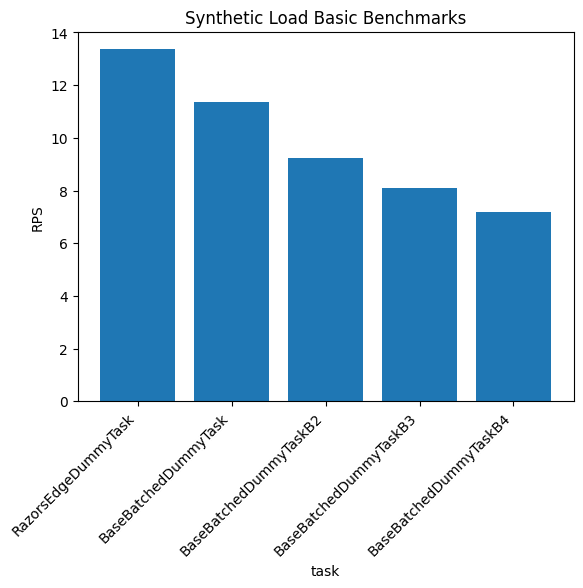
\includegraphics[width=\linewidth]{images_latex/Synthetic_Load_Basic_Benchmarks.png}

For the \texttt{BAAI/bge-m3} GPU workload, Razor\textquotesingle s Edge
achieved a throughput of 35.3 RPS (25\% higher than the baseline), with
a maximum allowed batch size of 16. For the real model workload, the
baseline strategy achieved a throughput of 28.2 RPS, with best
performance when the batch size was limited to 1. In this setting,
simple batching did not improve throughput.

\textbf{Figure 2:} \texttt{BAAI/bge-m3} GPU workload benchmark
comparison.

\textbf{Notebook source:}
\path{demos/real/gpu_benchmark_performance_comparison_basic.ipynb}.

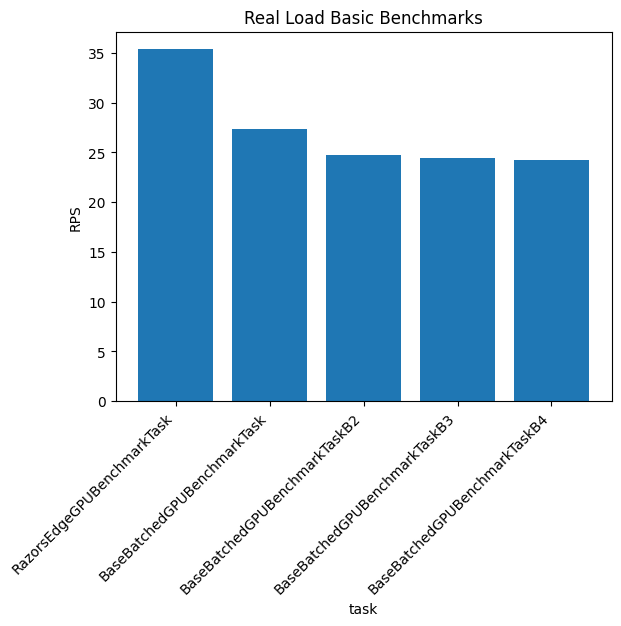
\includegraphics[width=\linewidth]{images_latex/Real_Load_Basic_Benchmarks.png}

For the \texttt{BAAI/bge-m3} GPU workload with limited token input,
Razor\textquotesingle s Edge achieved a throughput of 84.6 RPS (26\%
higher than the baseline with batch size = 10), with a maximum allowed
batch size of 16. For this limited-token workload, the baseline strategy
achieved a throughput of 67.4 RPS, with best performance at batch size =
10. Baseline batching improved throughput relative to the non-batched
baseline of 41.4 RPS (39\% lower than the baseline with batch size =
10).

\textbf{Figure 3:} \texttt{BAAI/bge-m3} GPU workload benchmark
comparison with limited tokens.

\textbf{Notebook source:}
\path{demos/real/gpu_benchmark_performance_comparison_basic_limited.ipynb}.

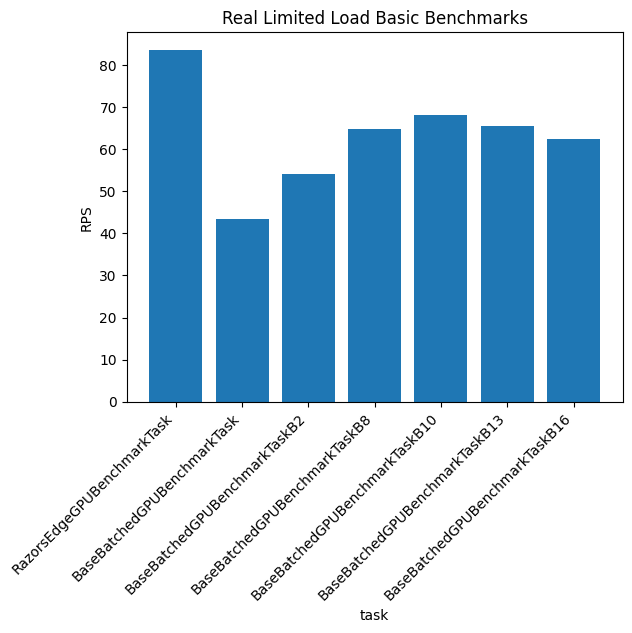
\includegraphics[width=\linewidth]{images_latex/Real_Limited_Load_Basic_Benchmarks.png}

For the \texttt{jinaai/jina-embeddings-v2-base-en} CPU workload,
Razor\textquotesingle s Edge achieved a throughput of 16.2 RPS (47\%
higher than the baseline with batch 2 and no batch), with a maximum
allowed batch size of 6. For this workload, the baseline strategy
achieved a throughput of 11.0 RPS, with best performance at batch size
2. Baseline batching marginally improved throughput relative to the
non-batched baseline of 10.5 RPS (5\% lower than the baseline with batch
size = 2).

\textbf{Figure 4:} Real \texttt{jinaai/jina-embeddings-v2-base-en} CPU
benchmark comparison.

\textbf{Notebook source:}
\path{demos/cpu/razors_edge_cpu_benchmark_task.py}.

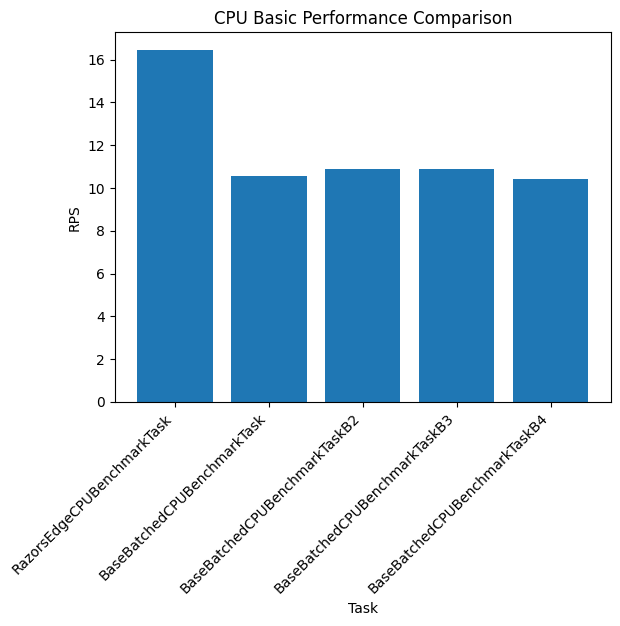
\includegraphics[width=\linewidth]{images_latex/CPU_Basic_Performance_Comparison.png}

For the synthetic workload, we compare the three outlined latency
objectives.

\textbf{Figure 5:} Synthetic latency comparison.

\textbf{Notebook source:}
\path{demos/synthetic/dummy_latency_comparison.ipynb}.

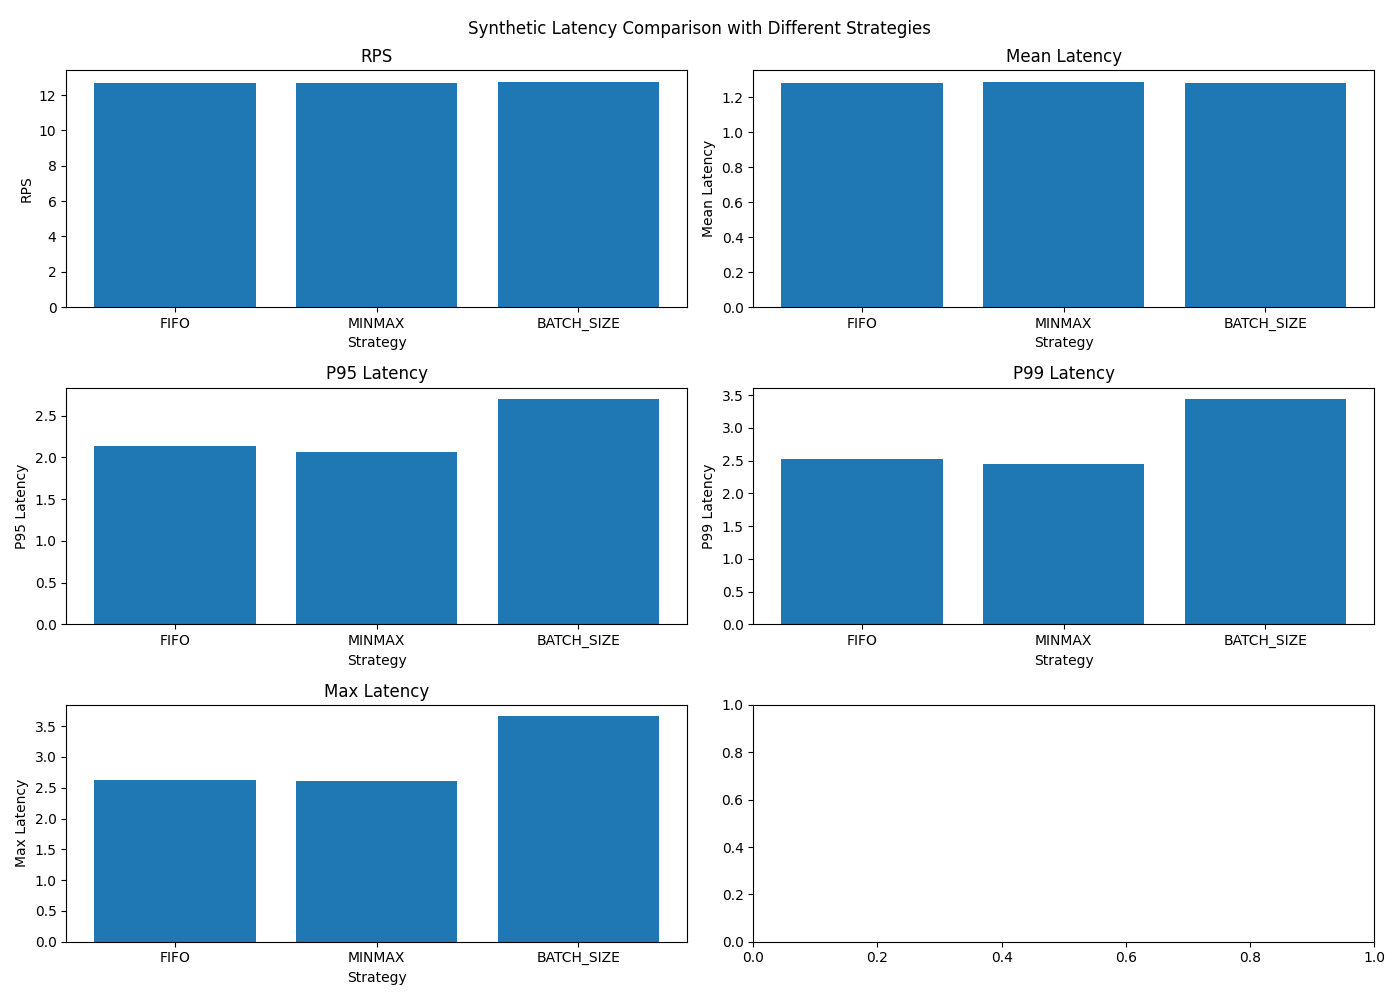
\includegraphics[width=\linewidth]{images_latex/Synthetic_Latency_Comparison_with_Different_Strategies.png}

For the \texttt{BAAI/bge-m3} GPU workload with limited tokens, we
compare the three outlined latency objectives.

\textbf{Figure 6:} Real \texttt{BAAI/bge-m3} GPU latency comparison.

\textbf{Notebook source:}
\path{demos/real/gpu_benchmark_limited_latency_comparison.ipynb}.

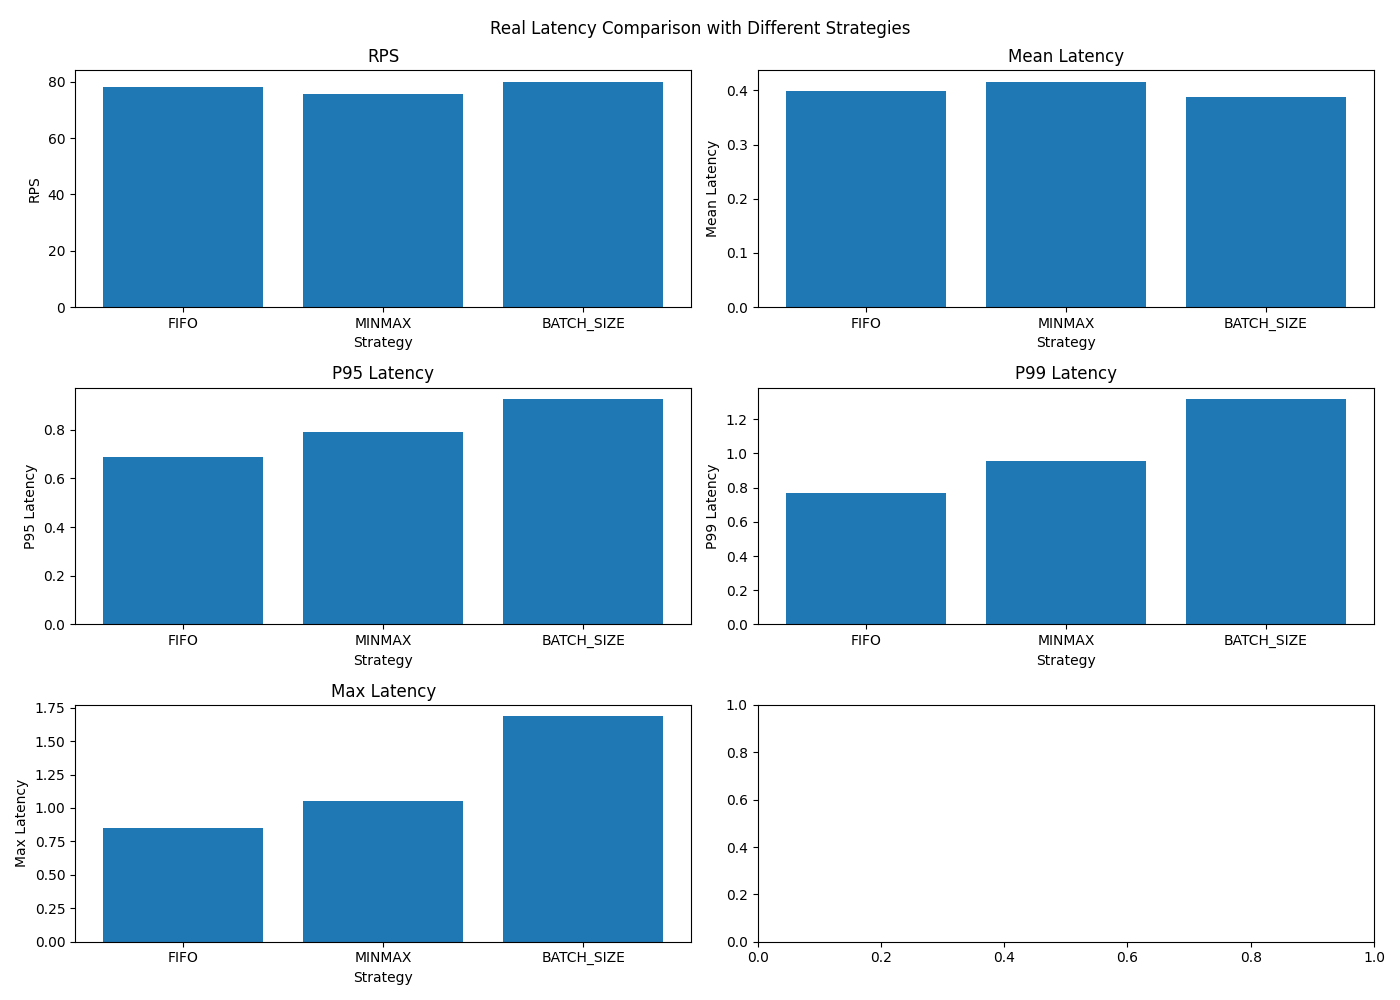
\includegraphics[width=\linewidth]{images_latex/Real_Latency_Comparison_with_Different_Strategies.png}

For the \texttt{jinaai/jina-embeddings-v2-base-en} CPU workload, we
compare the three outlined latency objectives.

\textbf{Figure 7:} Real \texttt{jinaai/jina-embeddings-v2-base-en} CPU
latency comparison.

\textbf{Notebook source:}
\path{demos/cpu/cpu_benchmark_latency_comparison.ipynb}.

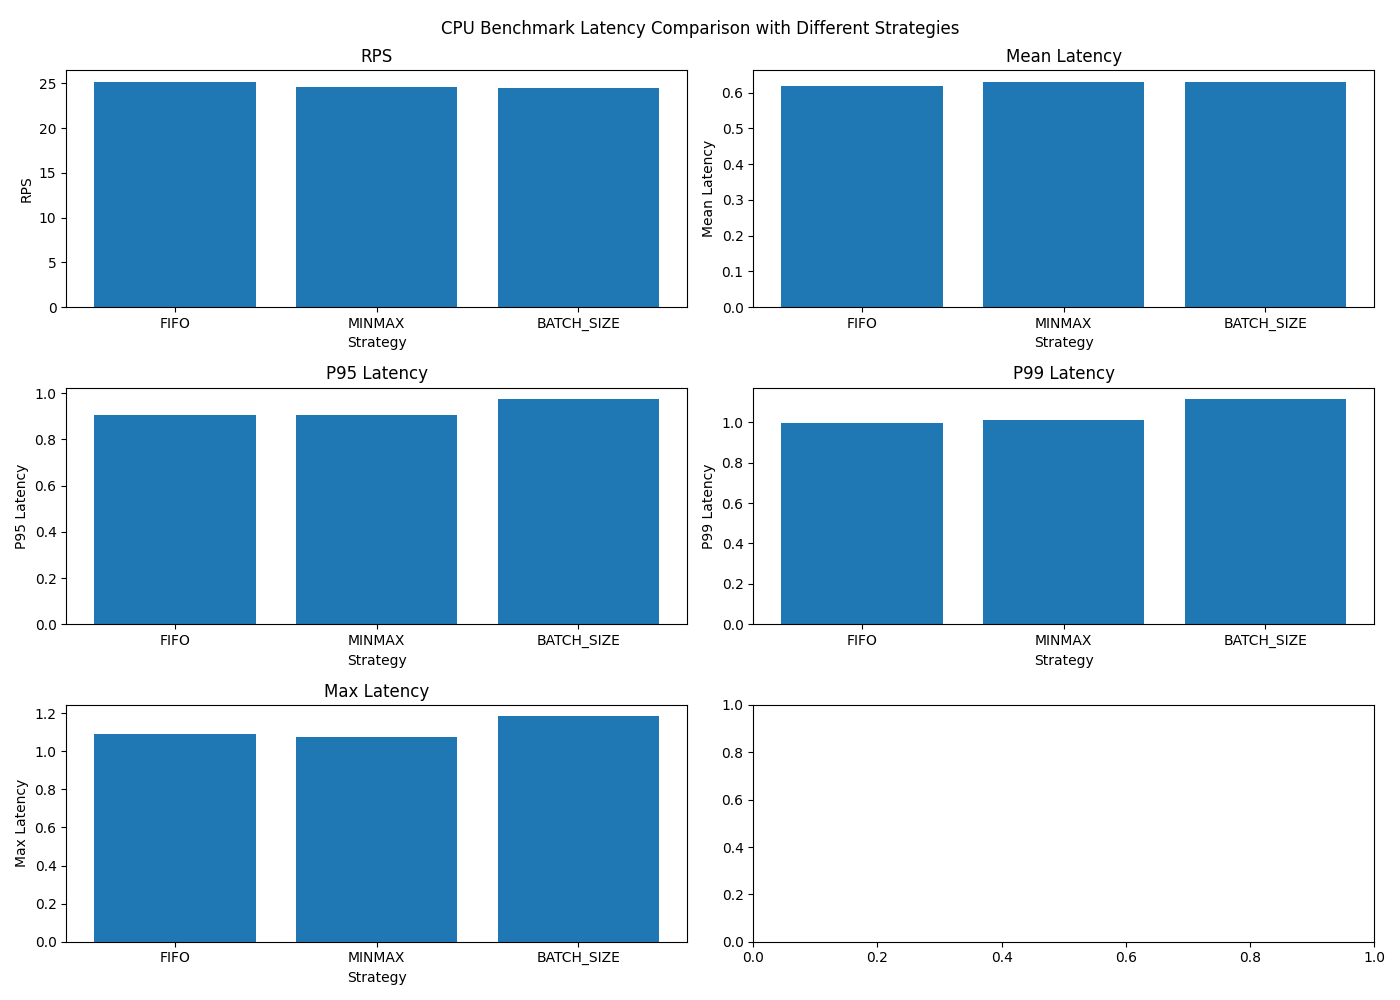
\includegraphics[width=\linewidth]{images_latex/CPU_Benchmark_Latency_Comparison_with_Different_Strategies.png}

\hypertarget{71-baseline-policy-definition}{%
\subsection{Baseline Policy
Definition}\label{71-baseline-policy-definition}}

The baseline in Section 7 is the \texttt{BaseBatchedComputeTask} policy
run under \texttt{ComputeExecutor}, with behavior as implemented:

\begin{itemize}
\tightlist
\item
  \textbf{FIFO oldest-first selection (no reordering/sorting):} each
  per-task queue is a Python \texttt{dict} keyed by
  \texttt{(operation\_id,\ queue\_time)} and consumed from iteration
  order; \texttt{choose\_fair\_queue} picks the queue whose first key is
  globally smallest, and \texttt{get\_batch\_ids\_list\_and\_batch}
  consumes from the first enqueued item onward. This preserves arrival
  order and does not apply size-based sorting.\\
  Implementation points:
  \begin{itemize}
  \tightlist
  \item
    \path{ComputeExecutor._InternalProcess.accumulate_data}
  \item
    \path{ComputeExecutor._InternalProcess.choose_fair_queue}
  \item
    \path{BaseBatchedComputeTask.get_batch_ids_list_and_batch}
  \end{itemize}
\item
  \textbf{Immediate dispatch on idle:} when all queues are empty,
  \texttt{accumulate\_data} blocks until at least one request arrives;
  the loop then immediately selects a fair queue, forms a batch, removes
  ids, and submits execution without any delay.\\
  Implementation points:
  \begin{itemize}
  \tightlist
  \item
    \path{ComputeExecutor._InternalProcess.__init__} main loop
  \item
    \path{ComputeExecutor._InternalProcess.accumulate_data}
  \end{itemize}
\item
  \textbf{Append until max batch size \texttt{n}:} baseline task
  variants implement \texttt{\_accept\_in\_batch} as
  \texttt{len(current\_batch)\ \textless{}\ self.max\_batch\_size}, so
  batching is a maximal prefix up to fixed cap \texttt{n}.\\
  Implementation points:
  \path{demos/synthetic/base\_batched\_dummy\_task.py} and
  \path{demos/real/base\_batched\_gpu\_benchmark\_task.py} (both
  define \texttt{max\_batch\_size} and this predicate), plus variant
  classes that set \texttt{n}.
\end{itemize}

\textbf{Exact baseline hyperparameter grids (\texttt{n}) used in Section
7 comparisons}

\begin{itemize}
\tightlist
\item
  \textbf{Synthetic basic benchmark grid:}
  \texttt{n\ \\in \ \{1,\ 2,\ 3,\ 4\}} (via \texttt{BaseBatchedDummyTask},
  \texttt{BaseBatchedDummyTaskB2}, \texttt{BaseBatchedDummyTaskB3},
  \texttt{BaseBatchedDummyTaskB4}).
\item
  \textbf{Real basic benchmark grid:} \texttt{n\ \\in \ \{1,\ 2,\ 3,\ 4\}}
  (via \texttt{BaseBatchedGPUBenchmarkTask},
  \texttt{BaseBatchedGPUBenchmarkTaskB2},
  \texttt{BaseBatchedGPUBenchmarkTaskB3},
  \texttt{BaseBatchedGPUBenchmarkTaskB4}).
\item
  \textbf{Real limited-token benchmark grid:}
  \texttt{n\ \\in \ \{1,\ 2,\ 8,\ 10,\ 13,\ 16\}}.
\end{itemize}

\textbf{Method used to choose reported baseline setting}

For each workload, we benchmark each candidate \texttt{n} over 5 runs
and report the mean throughput (RPS) of 5 runs. This selected setting is
the one reported in Section 7 for that workload.

\hypertarget{72-data}{%
\subsection{Data}\label{72-data}}

For throughput, every run is reported.

For latency, we report the mean across 5 runs (measured in the same
notebooks).

\hypertarget{throughput-data}{%
\paragraph{Throughput data}\label{throughput-data}}

\begin{table}[t]
\caption{Throughput data: Synthetic Load. Source file: \path{demos/synthetic/dummy_performance_comparison_basic.ipynb}}
\label{throughput-synthetic}
\vskip 0.15in
\begin{center}
\begin{small}
\begin{sc}
\resizebox{\columnwidth}{!}{%
\begin{tabular}{lccccccc}
\toprule
Configuration & Run 1 & Run 2 & Run 3 & Run 4 & Run 5 & Mean & Std Dev \\
\midrule
Razor\textquotesingle s Edge (MINMAX) & 13.3 & 13.3 & 13.2 & 13.3 & 13.2 & 13.3 & 0.05 \\
No batching & 11.4 & 11.3 & 11.4 & 11.4 & 11.4 & 11.4 & 0.04 \\
\bottomrule
\end{tabular}%
}
\end{sc}
\end{small}
\end{center}
\vskip -0.1in
\end{table}

\begin{table}[t]
\caption{Throughput data: BAAI/bge-m3 GPU Workload. Source file: \path{demos/real/gpu_benchmark_performance_comparison.ipynb}}
\label{throughput-gpu}
\vskip 0.15in
\begin{center}
\begin{small}
\begin{sc}
\resizebox{\columnwidth}{!}{%
\begin{tabular}{lccccccc}
\toprule
Configuration & Run 1 & Run 2 & Run 3 & Run 4 & Run 5 & Mean & Std Dev \\
\midrule
Razor\textquotesingle s Edge (MINMAX) & 35.8 & 35.5 & 36.3 & 34.4 & 34.4 & 35.3 & 0.76 \\
No batching & 27.9 & 28.1 & 27.6 & 29.0 & 28.4 & 28.2 & 0.48 \\
\bottomrule
\end{tabular}%
}
\end{sc}
\end{small}
\end{center}
\vskip -0.1in
\end{table}

\begin{table}[t]
\caption{Throughput data: BAAI/bge-m3 GPU Workload (Limited tokens). Source file: \path{demos/real/gpu_benchmark_performance_comparison.ipynb}}
\label{throughput-gpu-limited}
\vskip 0.15in
\begin{center}
\begin{small}
\begin{sc}
\resizebox{\columnwidth}{!}{%
\begin{tabular}{lccccccc}
\toprule
Configuration & Run 1 & Run 2 & Run 3 & Run 4 & Run 5 & Mean & Std Dev \\
\midrule
Razor\textquotesingle s Edge (MINMAX) & 85.1 & 82.8 & 83.3 & 86.0 & 85.9 & 84.6 & 1.33 \\
Baseline (BS=10) & 68.1 & 69.0 & 68.3 & 66.0 & 65.5 & 67.4 & 1.37 \\
No batching & 42.0 & 37.9 & 45.5 & 41.1 & 40.6 & 41.4 & 2.46 \\
\bottomrule
\end{tabular}%
}
\end{sc}
\end{small}
\end{center}
\vskip -0.1in
\end{table}

\begin{table}[t]
\caption{Throughput data: jinaai/jina-embeddings-v2-base-en CPU Workload. Source file: \path{demos/cpu/cpu_performance_comparison_basic.ipynb}}
\label{throughput-cpu}
\vskip 0.15in
\begin{center}
\begin{small}
\begin{sc}
\resizebox{\columnwidth}{!}{%
\begin{tabular}{lccccccc}
\toprule
Configuration & Run 1 & Run 2 & Run 3 & Run 4 & Run 5 & Mean & Std Dev \\
\midrule
Razor\textquotesingle s Edge (MINMAX) & 16.3 & 16.1 & 16.4 & 16.2 & 16.2 & 16.2 & 0.10 \\
Baseline (BS=2) & 11.0 & 10.9 & 11.0 & 11.0 & 10.9 & 11.0 & 0.05 \\
No batching & 10.5 & 10.8 & 10.5 & 10.2 & 10.7 & 10.5 & 0.21 \\
\bottomrule
\end{tabular}%
}
\end{sc}
\end{small}
\end{center}
\vskip -0.1in
\end{table}

\hypertarget{721-estimator-array-replay-validation}{%
\subsection{Estimator-Array Replay Validation}\label{721-estimator-array-replay-validation}}

We also replayed key Section 7 throughput claims using only the saved
estimator arrays and a saturated simulation harness.

The estimator arrays were generated using:

\begin{itemize}
\tightlist
\item
  \path{demos/scheduler_tests/save_estimators_for_simulation.ipynb}
\end{itemize}

Replay estimator files:

\begin{itemize}
\tightlist
\item
  \path{demos/scheduler_tests/estimator_arrays/est_store_synthetic.txt}
\item
  \path{demos/scheduler_tests/estimator_arrays/est_store_bge_m3.txt}
\item
  \path{demos/scheduler_tests/estimator_arrays/est_store_jina.txt}
\end{itemize}

Method:

\begin{itemize}
\tightlist
\item
  5 seeds (\texttt{{[}42,\ 43,\ 44,\ 45,\ 46{]}}), 20,000 requests per
  seed, queue cap = 16.
\item
  Baseline is FIFO arrival-order fixed-cap batching, sweeping all
  supported \texttt{n} values and selecting best mean-RPS baseline.
\item
  Best Razor\textquotesingle s Edge replay compares final strategies
  (\texttt{FIFO}, \texttt{MINMAX}, \texttt{BATCH\_SIZE}) on sorted+DP
  candidate chains.
\end{itemize}

\begin{table}[t]
\centering
\resizebox{\columnwidth}{!}{%
\begin{tabular}{@{}lrlrrr@{}}
\toprule\noalign{}
Workload & baseline RPS & Batch selection & Razor\textquotesingle s Edge
RPS & Replay uplift (\%) &
Hardware uplift (\%) \\
\midrule\noalign{}

\bottomrule\noalign{}

Synthetic & 11.348 & \texttt{BATCH\_SIZE} & 13.095 & 15.39 & 17.00 \\
\texttt{BAAI/bge-m3} (GPU) & 27.887 & \texttt{FIFO} &
37.490 & 34.44 & 26.00 \\
\texttt{jina-embeddings} &
3.488 & \texttt{BATCH\_SIZE} & 4.373 & 25.38 & 47.00 \\
\end{tabular}%
}
\end{table}

These replay values are reported raw from estimator-array simulation and
are intended as a consistency/sensitivity check alongside the end-to-end
runtime notebook measurements.

\hypertarget{722-ablative-study-estimator-replay}{%
\subsection{Ablative Study (Estimator
Replay)}\label{722-ablative-study-estimator-replay}}

We isolate each mechanism in the scheduling stack with the following
variants:

\begin{itemize}
\tightlist
\item
  \textbf{A}: baseline fixed-cap FIFO (unsorted queue).
\item
  \textbf{B}: sort-only fixed-cap FIFO (same \texttt{n} as variant A).
\item
  \textbf{C}: sort + DP + FIFO objective.
\item
  \textbf{D}: sort + DP + MINMAX objective.
\item
  \textbf{E}: sort + DP + BATCH\_SIZE objective.
\item
  \textbf{F}: sort + greedy batch-construction + MINMAX objective.
\end{itemize}

\begin{table}[t]
\centering
\resizebox{\columnwidth}{!}{%
\begin{tabular}{@{}lrrrrrrr@{}}
\toprule\noalign{}
Workload &\texttt{n} used for A/B & A mean RPS & B mean RPS & C
mean RPS & D mean RPS & E mean RPS & F mean RPS \\
\midrule\noalign{}

\bottomrule\noalign{}
Synthetic & 1 & 11.348 & 11.348 & 13.054 & 13.060 & 13.095 & 12.952 \\
\texttt{BAAI/bge-m3} replay & 3 & 27.887 & 27.924 & 37.490 & 37.173 &
36.601 & 31.368 \\
\texttt{jina-embeddings} replay & 1 & 3.488 & 3.488 &
4.370 & 4.370 & 4.373 & 4.121 \\
\end{tabular}%
}
\end{table}

Incremental mean-RPS deltas:

\begin{itemize}
\tightlist
\item
  Synthetic: \texttt{B-A\ =\ 0.000}, \texttt{D-B\ =\ 1.712},
  \texttt{C-D\ =\ -0.006}, \texttt{E-D\ =\ 0.034}.
\item
  \texttt{BAAI/bge-m3}: \texttt{B-A\ =\ 0.037}, \texttt{D-B\ =\ 9.249},
  \texttt{C-D\ =\ 0.317}, \texttt{E-D\ =\ -0.572}.
\item
  \texttt{jinaai/jina-embeddings-v2-base-en}: \texttt{B-A\ =\ 0.000},
  \texttt{D-B\ =\ 0.882}, \texttt{C-D\ =\ -0.000},
  \texttt{E-D\ =\ 0.003}.
\item
  Greedy(MINMAX)-vs-DP(MINMAX) (\texttt{F-D}): Synthetic
  \texttt{-0.108}, \texttt{BAAI/bge-m3} \texttt{-5.805},
  \texttt{jinaai/jina-embeddings-v2-base-en} \texttt{-0.250}.
\end{itemize}

This mechanism-isolation replay is included as a simulation-only
complement to the end-to-end runtime comparisons in Section 7.

\hypertarget{723-threats-to-validity-for-replay-results}{%
\subsection{Threats to Validity for Replay
Results}\label{723-threats-to-validity-for-replay-results}}

The estimator-array replay results in Section 7.2.1-7.2.2 should be
interpreted with the following constraints:

\begin{enumerate}
\def\labelenumi{\arabic{enumi}.}
\item
  \textbf{Simulation layer vs runtime system layer.}\\
  Replay uses calibrated estimator arrays and scheduler logic, but does
  not model framework/runtime effects such as Python overhead variance,
  CUDA stream contention, allocator behavior, and OS-level scheduling
  jitter.
\item
  \textbf{Closed-loop saturated queueing only.}\\
  The replay fills queues to capacity each scheduler loop. This is
  useful for stress testing batching behavior but does not cover
  open-loop arrival processes, burstiness, or non-stationary traffic.
\item
  \textbf{Sorting-sensitive latency artifacts in ablation.}\\
  The sort-only ablation variant changes queue order, which can produce
  latency changes that reflect reordering policy rather than pure
  compute-efficiency gains.
\item
  \textbf{Baseline family scope.}\\
  Replay baselines are fixed-cap FIFO families. These are valid
  operational baselines for this repository but are not exhaustive
  across all production serving policies.
\end{enumerate}

Accordingly, Section 7.2 is presented as a reproducible
sensitivity/consistency analysis, while end-to-end notebook measurements
remain the primary empirical evidence for absolute throughput and
latency claims.

\hypertarget{73-hardware-and-software}{%
\subsection{Hardware and
Software}\label{73-hardware-and-software}}

\hypertarget{hardware-and-os}{%
\paragraph{Hardware and OS}\label{hardware-and-os}}

Experiments were conducted on an ASUS ROG Zephyrus Duo 16 laptop.

\begin{itemize}
\tightlist
\item
  CPU: AMD Ryzen 9 6900HX (16 threads) (power limits: SPL 20W, sPPT 20W,
  fPPT 25W)
\item
  GPU: NVIDIA RTX 3080 Ti Laptop GPU (835 MHz fixed max clock, 185 MHz
  core OC, 210 MHz memory OC, 5 W dynamic boost, 80\\degree{}C temperature
  target)
\item
  OS: Windows 24H2 IoT with AtlasOS modifications
\item
  Cooling: maximum fan speeds; no thermal throttling observed
\end{itemize}

The most stable practical environment was used, with no background
application load and Python run at high process priority (using
\texttt{psutil}) to improve timing stability. Graphs/figures shown are
least-noisy representative runs for visual readability, while all
throughput values reported in text are means across 5 runs per setting.

\hypertarget{software}{%
\paragraph{Software}\label{software}}

Python 3.14.3 (\texttt{pip\ list} output):

\begin{verbatim}
Package                   Version
------------------------- ------------
accelerate                1.13.0
annotated-doc             0.0.4
anyio                     4.12.1
argon2-cffi               25.1.0
argon2-cffi-bindings      25.1.0
arrow                     1.4.0
asttokens                 3.0.1
async-lru                 2.3.0
attrs                     26.1.0
babel                     2.18.0
beautifulsoup4            4.14.3
bleach                    6.3.0
certifi                   2026.2.25
cffi                      2.0.0
charset-normalizer        3.4.6
click                     8.3.1
colorama                  0.4.6
comm                      0.2.3
contourpy                 1.3.3
coverage                  7.13.5
cycler                    0.12.1
debugpy                   1.8.20
decorator                 5.2.1
defusedxml                0.7.1
executing                 2.2.1
fastjsonschema            2.21.2
filelock                  3.25.2
flatbuffers               25.12.19
fonttools                 4.62.1
fqdn                      1.5.1
fsspec                    2026.2.0
h11                       0.16.0
hf-xet                    1.4.2
httpcore                  1.0.9
httpx                     0.28.1
huggingface_hub           0.36.2
idna                      3.11
ipykernel                 7.2.0
ipython                   9.11.0
ipython_pygments_lexers   1.1.1
ipywidgets                8.1.8
isoduration               20.11.0
jedi                      0.19.2
Jinja2                    3.1.6
joblib                    1.5.3
json5                     0.13.0
jsonpointer               3.0.0
jsonschema                4.26.0
jsonschema-specifications 2025.9.1
jupyter                   1.1.1
jupyter_client            8.8.0
jupyter-console           6.6.3
jupyter_core              5.9.1
jupyter-events            0.12.0
jupyter-lsp               2.3.0
jupyter_server            2.17.0
jupyter_server_terminals  0.5.4
jupyterlab                4.5.6
jupyterlab_pygments       0.3.0
jupyterlab_server         2.28.0
jupyterlab_widgets        3.0.16
kiwisolver                1.5.0
lark                      1.3.1
llvmlite                  0.46.0
markdown-it-py            4.0.0
MarkupSafe                3.0.3
matplotlib                3.10.8
matplotlib-inline         0.2.1
mdurl                     0.1.2
mistune                   3.2.0
ml_dtypes                 0.5.4
mpmath                    1.3.0
nbclient                  0.10.4
nbconvert                 7.17.0
nbformat                  5.10.4
nest-asyncio              1.6.0
networkx                  3.6.1
notebook                  7.5.5
notebook_shim             0.2.4
numba                     0.64.0
numpy                     2.4.3
onnx                      1.20.1
onnxruntime               1.24.4
optimum                   2.1.0
optimum-onnx              0.1.0
packaging                 25.0
pandocfilters             1.5.1
parso                     0.8.6
pillow                    12.1.1
pip                       26.0.1
platformdirs              4.9.4
prometheus_client         0.24.1
prompt_toolkit            3.0.52
protobuf                  7.34.1
psutil                    7.2.2
pure_eval                 0.2.3
pycparser                 3.0
Pygments                  2.19.2
pyparsing                 3.3.2
python-dateutil           2.9.0.post0
python-json-logger        4.0.0
pywinpty                  3.0.3
PyYAML                    6.0.3
pyzmq                     27.1.0
referencing               0.37.0
regex                     2026.2.28
requests                  2.32.5
rfc3339-validator         0.1.4
rfc3986-validator         0.1.1
rfc3987-syntax            1.1.0
rich                      14.3.3
rpds-py                   0.30.0
safetensors               0.7.0
scikit-learn              1.8.0
scipy                     1.17.1
Send2Trash                2.1.0
setuptools                80.10.2
shellingham               1.5.4
six                       1.17.0
soupsieve                 2.8.3
stack-data                0.6.3
sympy                     1.14.0
terminado                 0.18.1
threadpoolctl             3.6.0
tinycss2                  1.4.0
tokenizers                0.22.2
torch                     2.10.0+cu126
tornado                   6.5.5
tqdm                      4.67.3
traitlets                 5.14.3
transformers              4.57.6
typer                     0.24.1
typing_extensions         4.15.0
tzdata                    2025.3
uri-template              1.3.0
urllib3                   2.6.3
wcwidth                   0.6.0
webcolors                 25.10.0
webencodings              0.5.1
websocket-client          1.9.0
wheel                     0.46.3
widgetsnbextension        4.0.15
\end{verbatim}

\hypertarget{74-workloads}{%
\subsection{Workloads}\label{74-workloads}}

Synthetic workload: We construct a dummy model where processing time is
a function of input size and batch size. This isolates batching effects
and enables clear visualization of performance structure. The synthetic
workload uses an accurate delay based on batch input size. Final
strategy comparisons use FIFO, MINMAX, and GUARDED\_BATCH\_SIZE.
Throughput numbers use MINMAX (recommended default). Real GPU workload:
We evaluate a batched inference pipeline using the \texttt{BAAI/bge-m3}
model on GPU. CPU workload: We evaluate the shape of the batching
performance contours of \texttt{jinaai/jina-embeddings-v2-base-en} on
CPU.

Requests were created using uniform-random characters with varying
lengths:

\begin{itemize}
\tightlist
\item
  1 to 1000 characters for the synthetic task
\item
  1 to 1300 chars (corresponding to 1 to 1000 tokens) for the real task
  \texttt{BAAI/bge-m3}
\item
  1 to 500 chars (corresponding to 1 to 400 tokens) for the limited real
  task \texttt{BAAI/bge-m3}
\item
  1 to 200 chars for the CPU task
  \texttt{jinaai/jina-embeddings-v2-base-en}
\end{itemize}

\hypertarget{75-throughput-under-increasing-load}{%
\subsection{Throughput under Increasing
Load}\label{75-throughput-under-increasing-load}}

We next evaluate system throughput as a function of load by varying the
number of concurrent requests.

The comparison figures in this section show Razor\textquotesingle s Edge
against the baseline dynamic batching strategy. The baseline exhibits
approximately constant throughput as load increases, reflecting its
reliance on fixed-size aggregation without improved batching quality. In
contrast, Razor\textquotesingle s Edge shows increasing throughput with
load up to saturation.

\hypertarget{graphs}{%
\paragraph{Graphs}\label{graphs}}

\hypertarget{synthetic}{%
\subparagraph{Synthetic}\label{synthetic}}

\textbf{Figure 8:} Baseline scheduler throughput vs. parallelism
(synthetic workload).

\textbf{Notebook source:}
\path{demos/synthetic/dummy_performance_comparison.ipynb}.

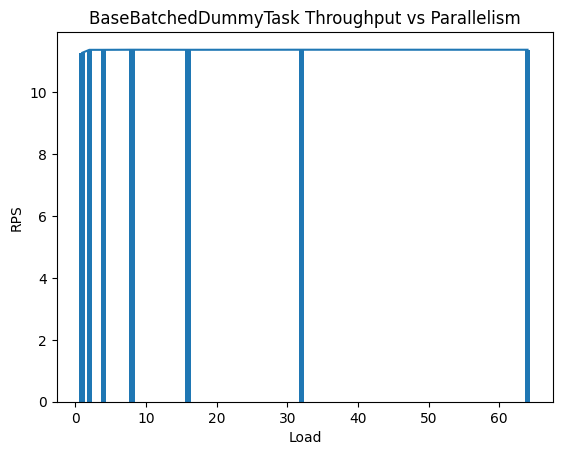
\includegraphics[width=\linewidth]{images_latex/BaseBatchedDummyTask_Throughput_vs_Parallelism.png}

\textbf{Figure 9:} Razor\textquotesingle s Edge scheduler throughput vs.
parallelism (synthetic workload).

\textbf{Notebook source:}
\path{demos/synthetic/dummy_performance_comparison.ipynb}.

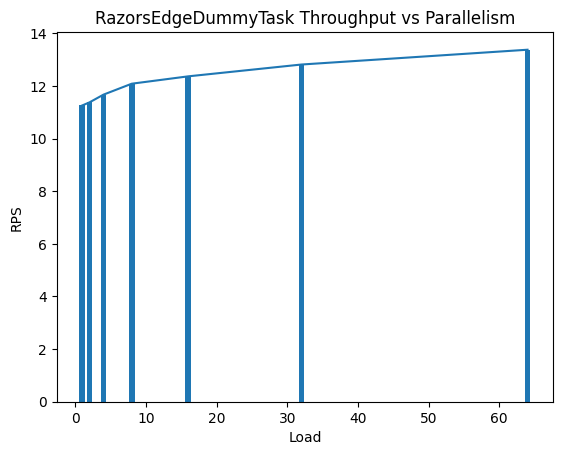
\includegraphics[width=\linewidth]{images_latex/RazorsEdgeDummyTask_Throughput_vs_Parallelism.png}

\textbf{Figure 10:} Direct throughput comparison of baseline and
Razor\textquotesingle s Edge (synthetic workload).

\textbf{Notebook source:}
\path{demos/synthetic/dummy_performance_comparison.ipynb}.

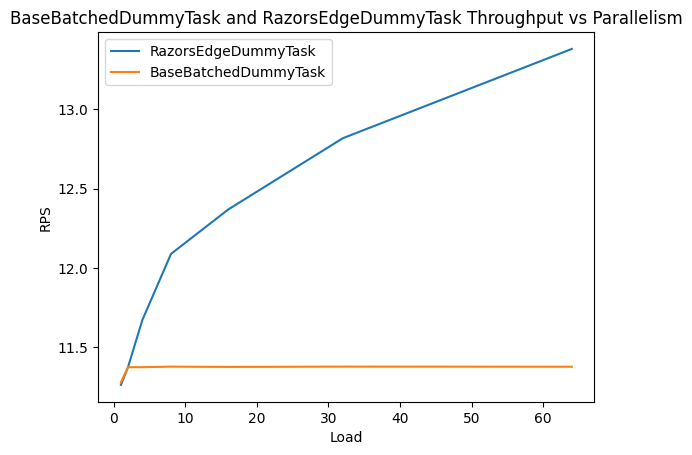
\includegraphics[width=\linewidth]{images_latex/BaseBatchedDummyTask_and_RazorsEdgeDummyTask_Throughput_vs_Parallelism.png}

\hypertarget{baaibge-m3-gpu-workload}{%
\subparagraph{BAAI/bge-m3 GPU workload}\label{baaibge-m3-gpu-workload}}

\textbf{Figure 11:} Baseline scheduler throughput vs. parallelism
(\texttt{BAAI/bge-m3} GPU workload).

\textbf{Notebook source:}
\path{demos/real/gpu_benchmark_performance_comparison.ipynb}.

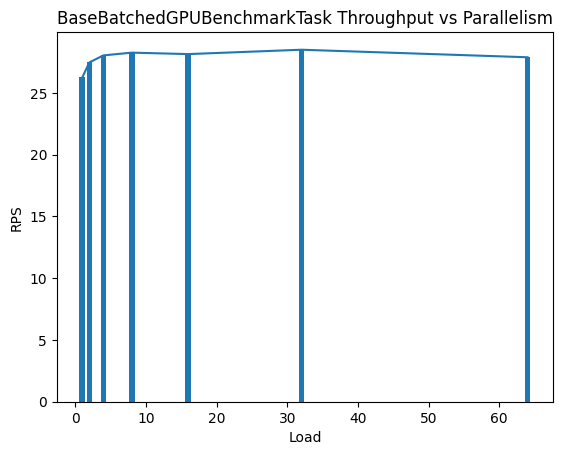
\includegraphics[width=\linewidth]{images_latex/BaseBatchedGPUBenchmarkTask_Throughput_vs_Parallelism.png}

\textbf{Figure 12:} Razor\textquotesingle s Edge scheduler throughput
vs. parallelism (\texttt{BAAI/bge-m3} GPU workload).

\textbf{Notebook source:}
\path{demos/real/gpu_benchmark_performance_comparison.ipynb}.

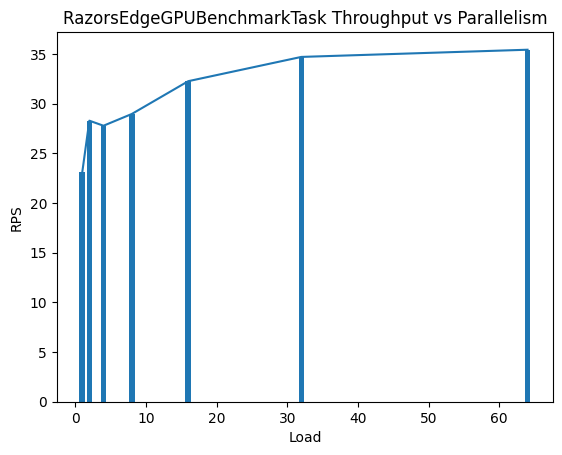
\includegraphics[width=\linewidth]{images_latex/RazorsEdgeGPUBenchmarkTask_Throughput_vs_Parallelism.png}

\textbf{Figure 13:} Direct throughput comparison of baseline and
Razor\textquotesingle s Edge (\texttt{BAAI/bge-m3} GPU workload).

\textbf{Notebook source:}
\path{demos/real/gpu_benchmark_performance_comparison.ipynb}.

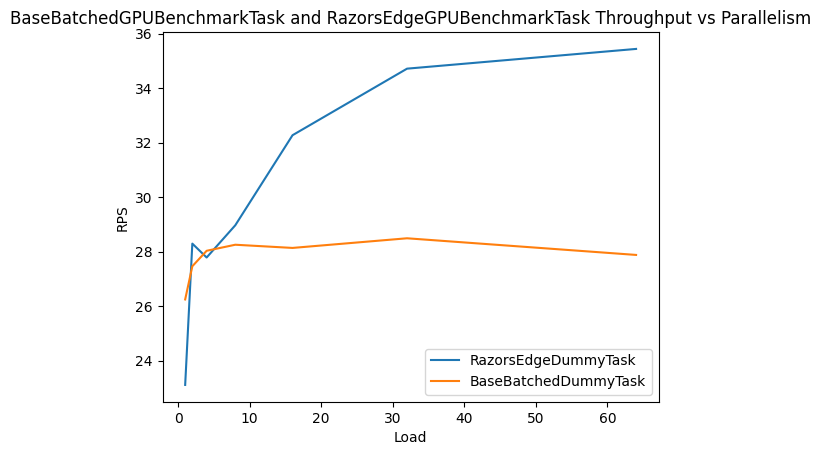
\includegraphics[width=\linewidth]{images_latex/BaseBatchedGPUBenchmarkTask_and_RazorsEdgeGPUBenchmarkTask_Throughput_vs_Parallelism.png}

\hypertarget{jinaaijina-embeddings-v2-base-en-cpu-workload-1}{%
\subparagraph{jinaai/jina-embeddings-v2-base-en CPU
workload}\label{jinaaijina-embeddings-v2-base-en-cpu-workload-1}}

\textbf{Figure 14:} Baseline scheduler throughput vs. parallelism
(\texttt{jinaai/jina-embeddings-v2-base-en} CPU workload).

\textbf{Notebook source:}
\path{demos/cpu/cpu_performance_comparison.ipynb}.

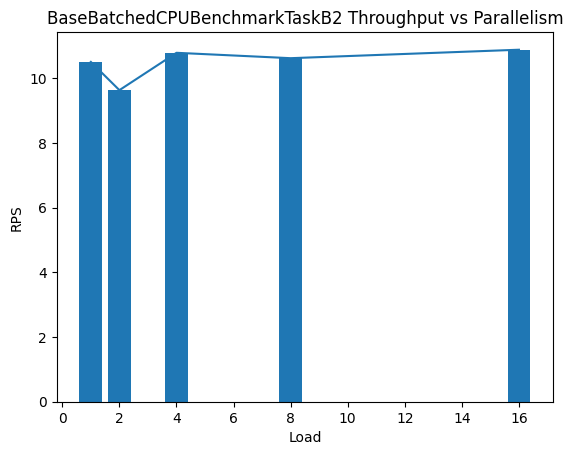
\includegraphics[width=\linewidth]{images_latex/BaseBatchedCPUBenchmarkTaskB2_Throughput_vs_Parallelism.png}

\textbf{Figure 15:} Razor\textquotesingle s Edge scheduler throughput
vs. parallelism (\texttt{jinaai/jina-embeddings-v2-base-en} CPU
workload).

\textbf{Notebook source:}
\path{demos/cpu/cpu_performance_comparison.ipynb}.

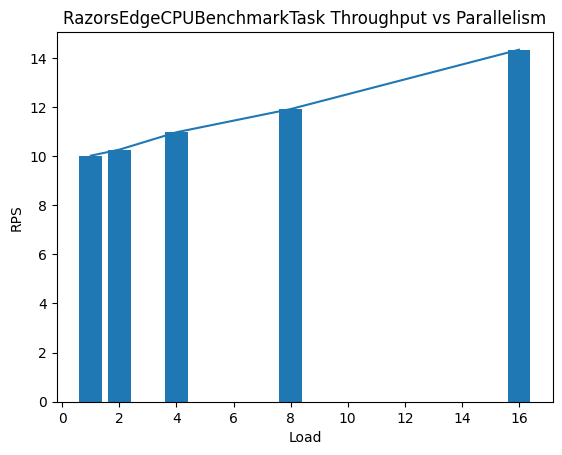
\includegraphics[width=\linewidth]{images_latex/RazorsEdgeCPUBenchmarkTask_Throughput_vs_Parallelism.png}

\textbf{Figure 16:} Direct throughput comparison of baseline and
Razor\textquotesingle s Edge (\texttt{jinaai/jina-embeddings-v2-base-en}
CPU workload).

\textbf{Notebook source:}
\path{demos/cpu/cpu_performance_comparison.ipynb}.

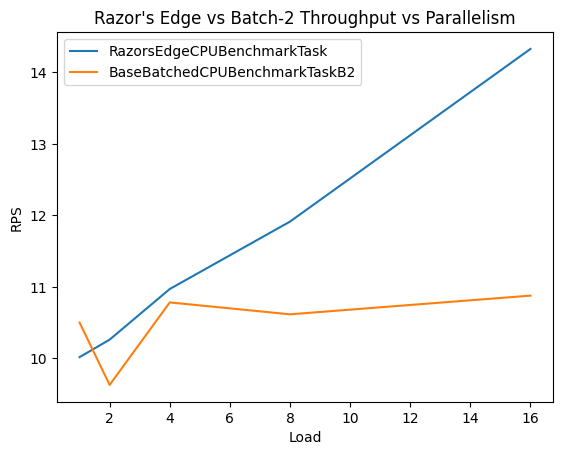
\includegraphics[width=\linewidth]{images_latex/Razors_Edge_vs_Batch-2_Throughput_vs_Parallelism.png}

\hypertarget{reasoning}{%
\paragraph{Reasoning}\label{reasoning}}

This effect arises because larger queue sizes enable better sorting of
input sizes, allowing the scheduler to construct more efficient batches.
As concurrency increases, the dynamic program has greater flexibility to
select near-optimal partitions, improving overall hardware utilization.

We observe this trend clearly in both synthetic and real workloads.
These results demonstrate that Razor\textquotesingle s Edge can exploit
queue depth to improve batching efficiency, partially offsetting
increased-load effects.

\hypertarget{76-razors-edge-structure-in-batching-efficiency}{%
\subsection{Razor\textquotesingle s Edge Structure in Batching
Efficiency}\label{76-razors-edge-structure-in-batching-efficiency}}

We next describe a visualization method used in this work to measure
batching efficiency structure.

For a fixed target size (N), define a queue (Q\_\{x,y,N\}) of exactly
(N) requests with input sizes drawn uniformly from ({[}x,y{]})
(inclusive). For each ((x,y)) pair:

\begin{enumerate}
\def\labelenumi{\arabic{enumi}.}
\tightlist
\item
  Compute \textbf{forced-(N)} time, where all (N) requests are forced
  into one batch of size (N):
\end{enumerate}

\begin{equation}
T^{\mathrm{forced}}_N(x,y)
\end{equation}

\begin{enumerate}
\def\labelenumi{\arabic{enumi}.}
\setcounter{enumi}{1}
\tightlist
\item
  Compute \textbf{dynamic-((N-1))} best-case time using the same DP
  partitioning method introduced earlier, but with maximum allowed batch
  size (N-1):
\end{enumerate}

\begin{equation}
T^{\mathrm{dynamic}}_{N-1}(x,y)
\end{equation}

\begin{enumerate}
\def\labelenumi{\arabic{enumi}.}
\setcounter{enumi}{2}
\tightlist
\item
  Form the efficiency ratio:
\end{enumerate}

\begin{equation}
R_N(x,y)=\frac{T^{\mathrm{forced}}_N(x,y)}{T^{\mathrm{dynamic}}_{N-1}(x,y)}
\end{equation}

We then plot a grayscale heatmap over ((x,y)), with (x) on one axis and
(y) on the other, using (R\_N(x,y)) as intensity. We additionally draw
contour lines at:

\begin{equation}
R_N(x,y)\in\{0.85,\;0.9,\;0.95,\;1.0\}
\end{equation}

to visualize transitions in batching efficiency.

Interpretation:

\begin{itemize}
\tightlist
\item
  (\(R_N(x,y) \ll 1\)): forcing batch size \(N\) is
  substantially more efficient than the best dynamic strategy restricted
  to max size (N-1).
\item
  (\(R_N(x,y) \approx 1\)): little to no efficiency gain from
  allowing (N) instead of (N-1).
\item
  The contour transition region forms the observed
  "razor\textquotesingle s edge" shape.
\end{itemize}

On the synthetic workload, these contours show that smaller inputs
permit broader size mixing while larger inputs require tighter
within-batch uniformity. In this setup, this trend is consistent with a
transition from memory-dominated to compute-dominated behavior.

In the real \texttt{BAAI/bge-m3} GPU workload, we observe a
qualitatively similar contour trend with higher measurement noise. In
the real \texttt{jinaai/jina-embeddings-v2-base-en} CPU workload, we
again observe a similar contour structure, with a narrower
high-efficiency region consistent with stronger compute-bound penalties
for mismatch.

These measured contour structures support applicability to the evaluated
workload class (variable-size batched inference with calibrated
estimators). We do not claim the same structure for all untested models
and hardware.

\textbf{Figure 17:} Improvement from allowing variable batch sizes
(synthetic task performance contours).

\textbf{Notebook source:}
\path{demos/synthetic/razors_edge_dummy_graphs.ipynb}.

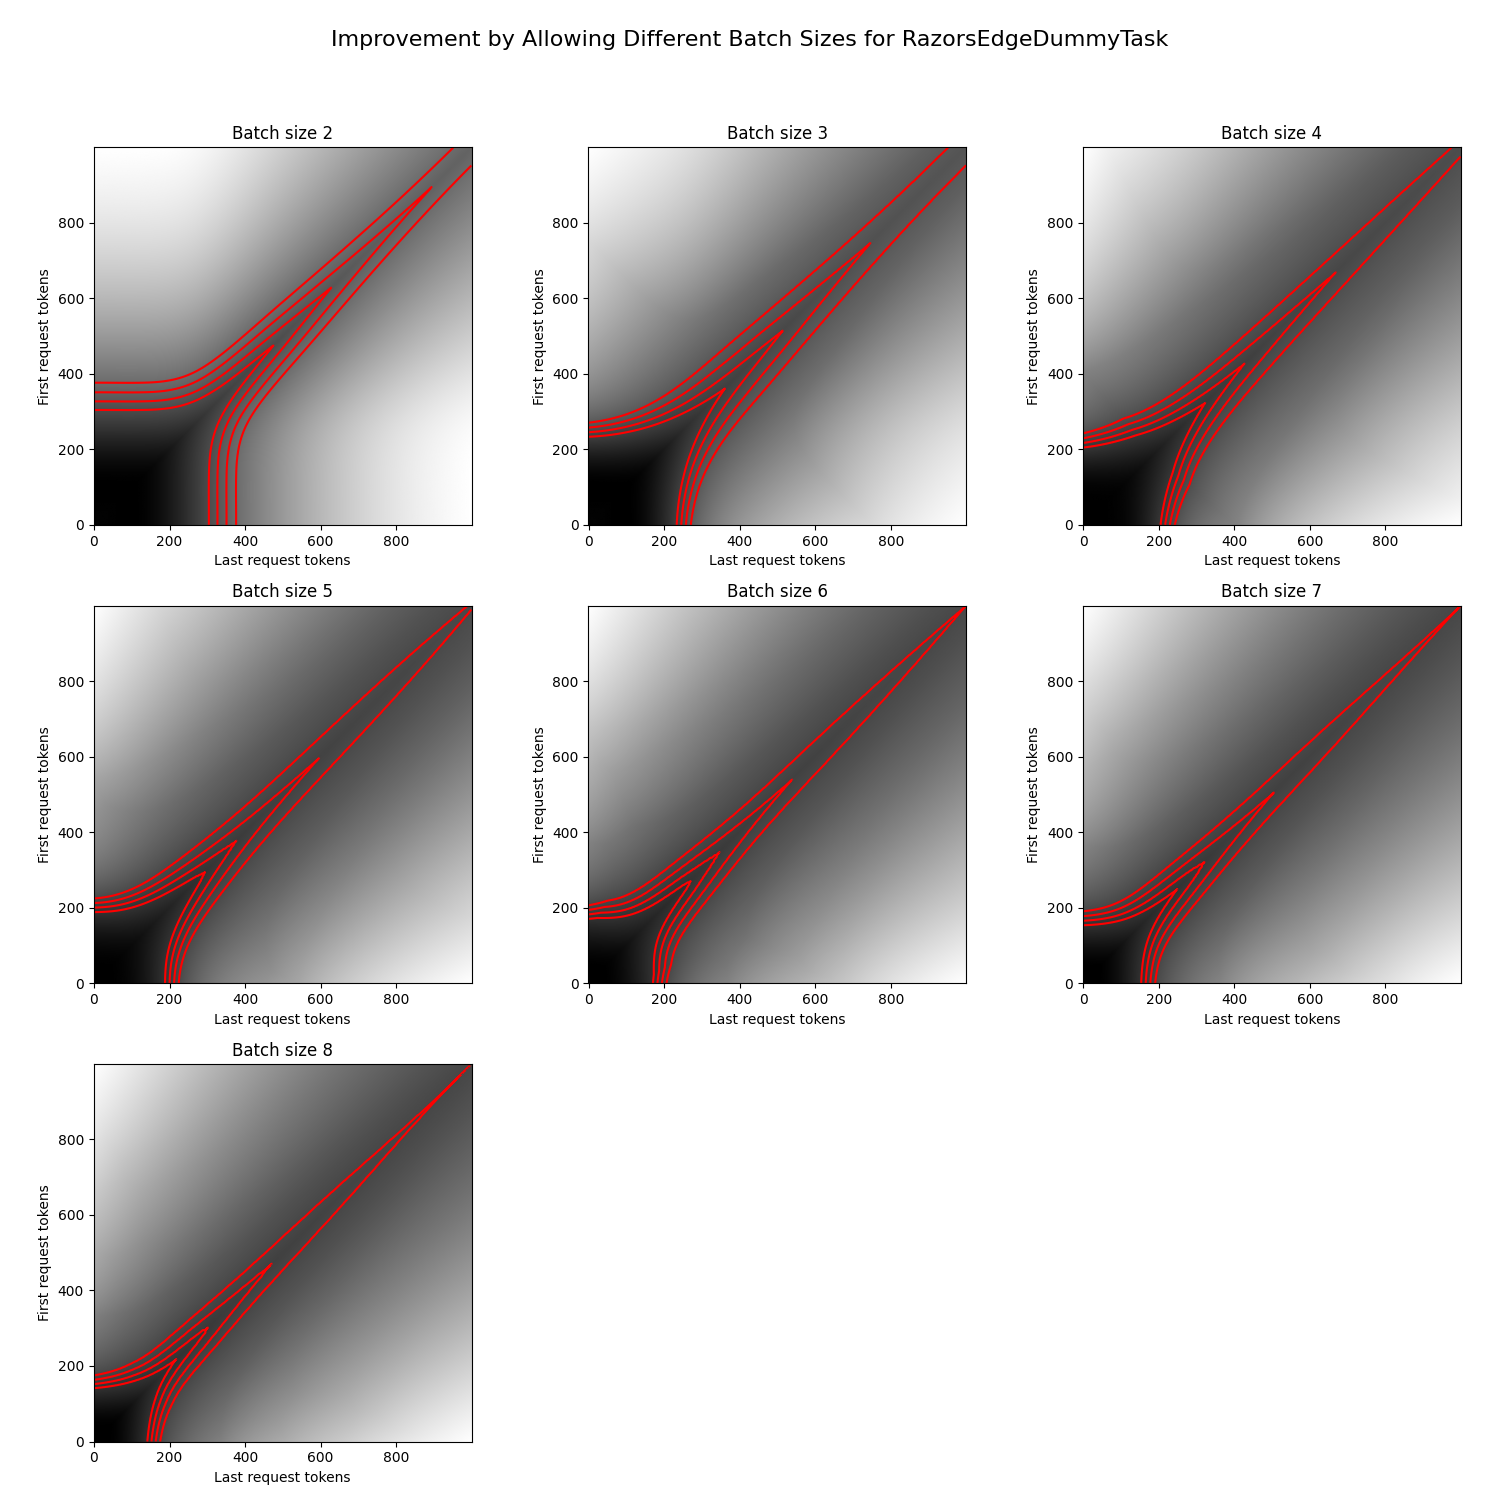
\includegraphics[width=\linewidth]{images_latex/Improvement_by_Allowing_Different_Batch_Sizes_for_RazorsEdgeDummyTask.png}

\textbf{Figure 18:} Improvement from allowing variable batch sizes
(real-model GPU performance contours).

\textbf{Notebook source:}
\path{demos/real/razors_edge_gpu_benchmark_graphs.ipynb}.

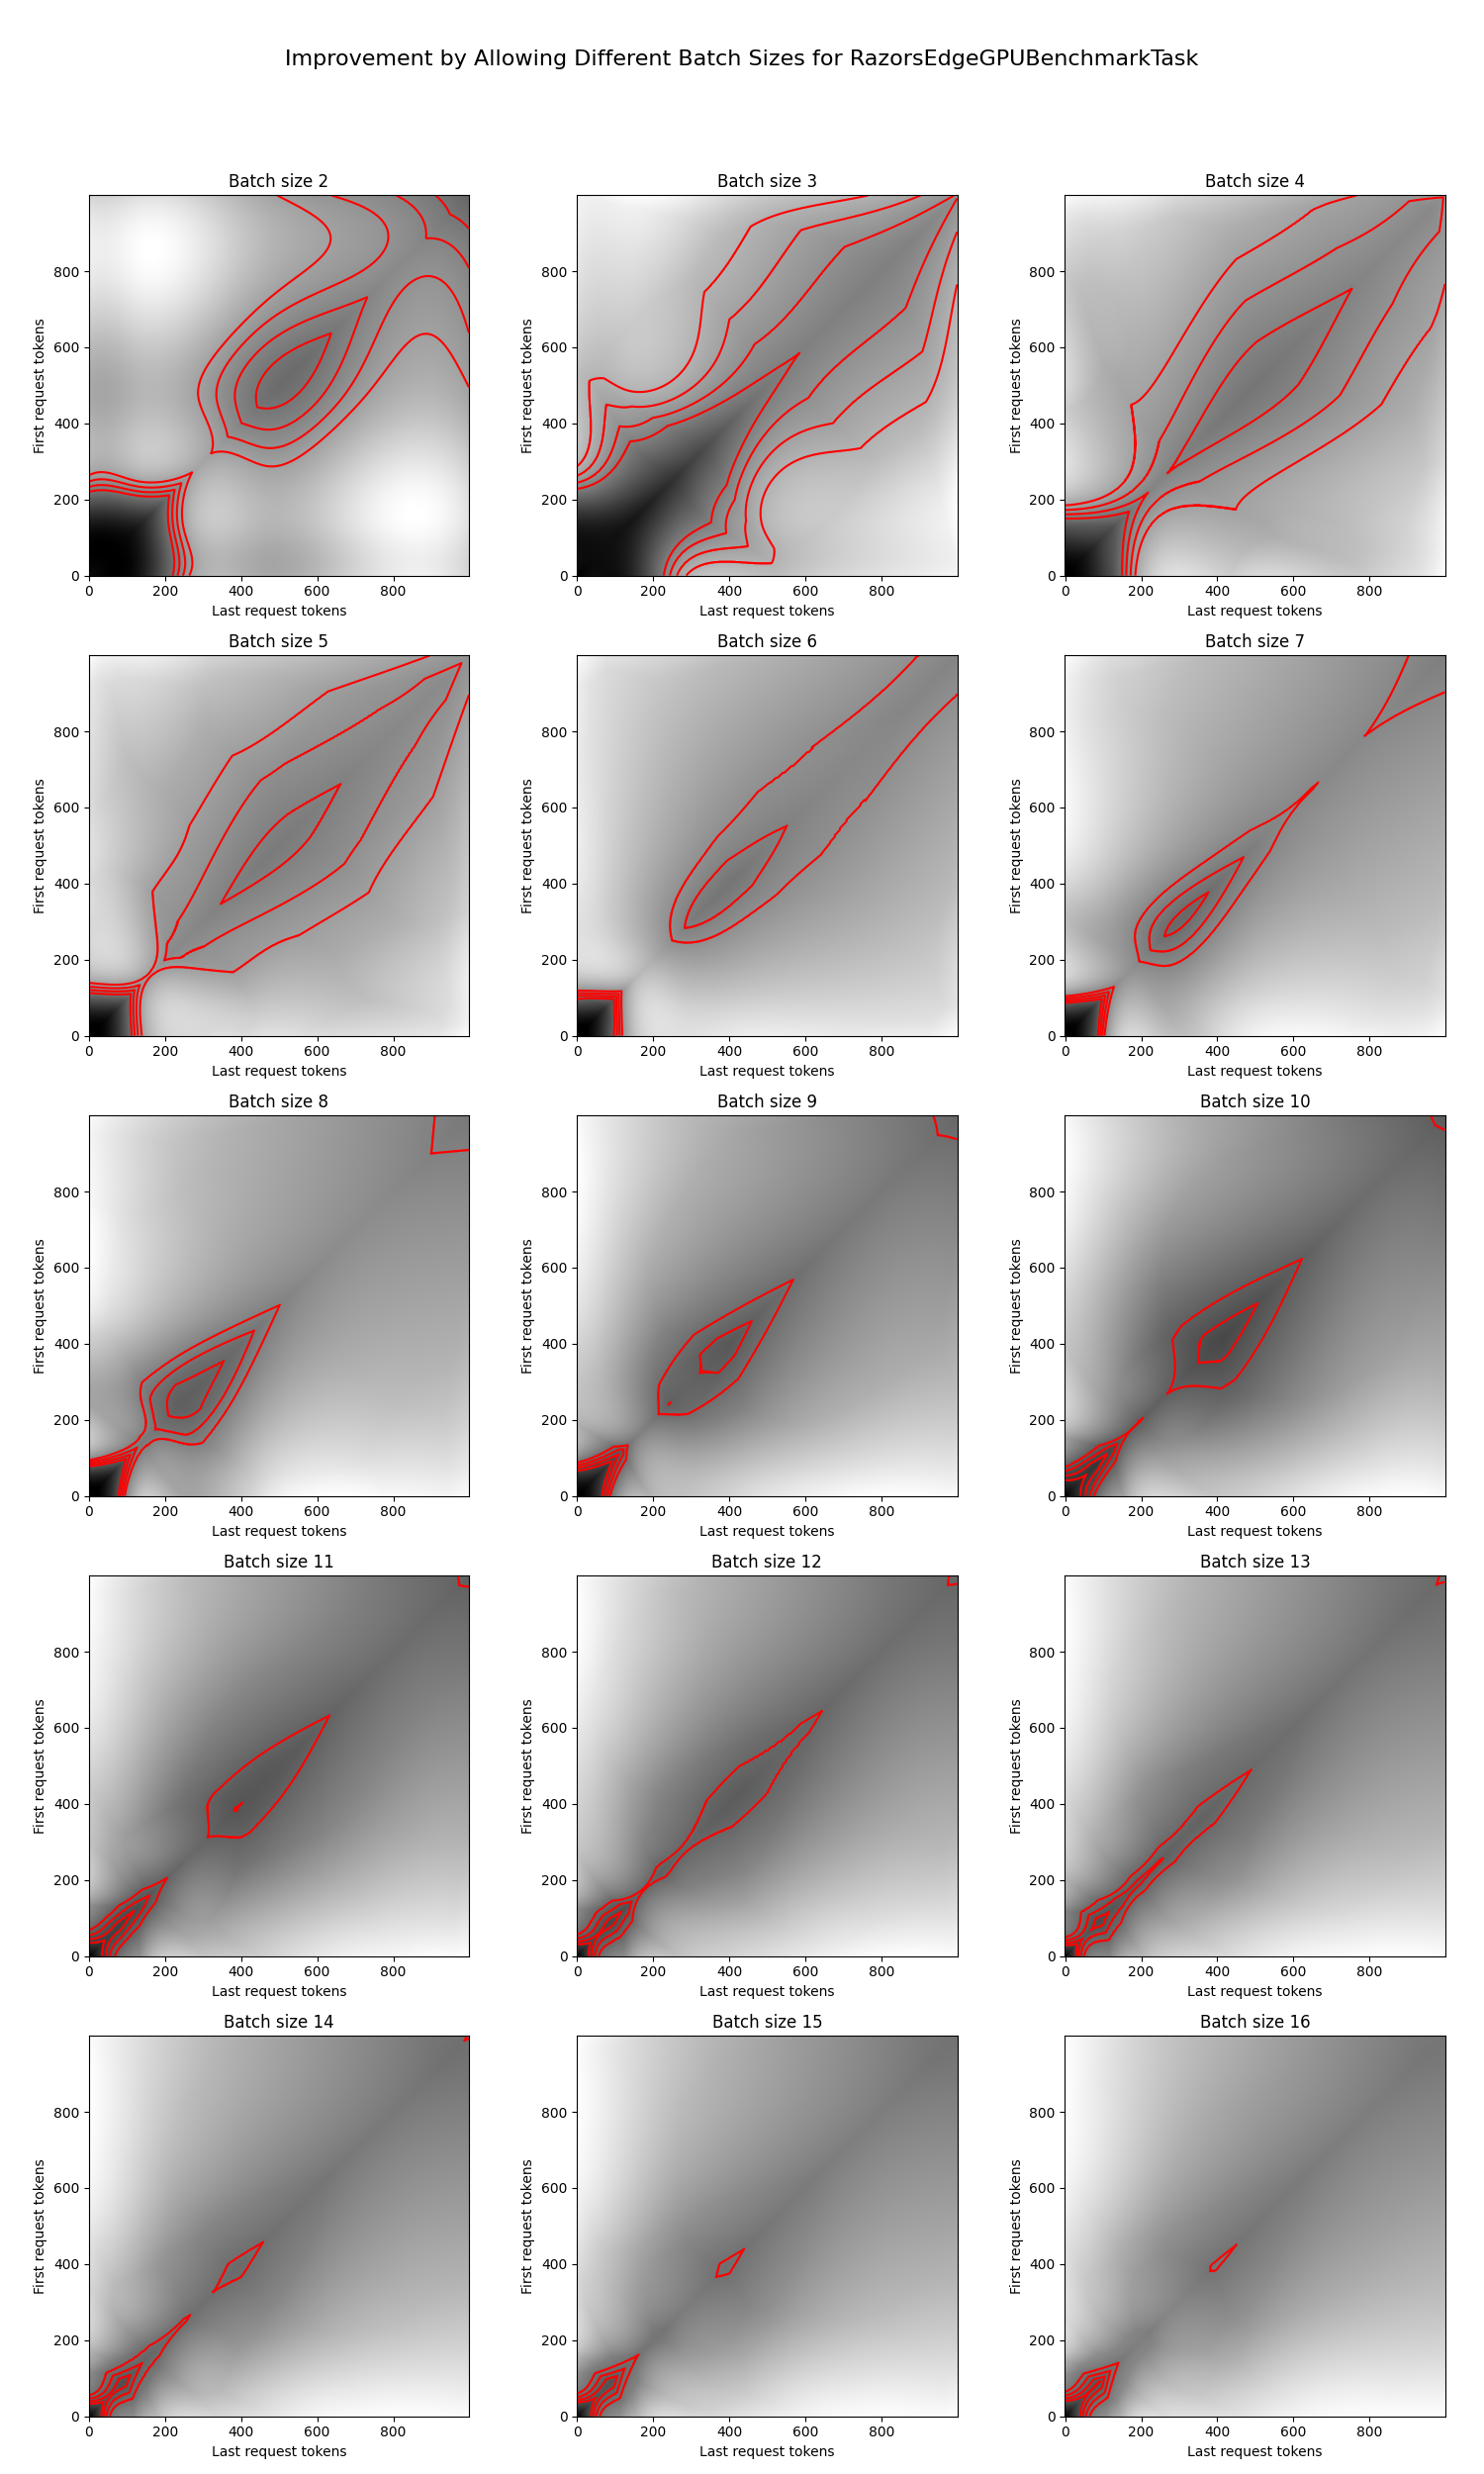
\includegraphics[width=\linewidth]{images_latex/Improvement_by_Allowing_Different_Batch_Sizes_for_RazorsEdgeGPUBenchmarkTask.png}

\textbf{Figure 19:} Improvement from allowing variable batch sizes
(real-model CPU performance contours).

\textbf{Notebook source:}
\path{demos/cpu/razors_edge_cpu_benchmark_graphs.ipynb}.

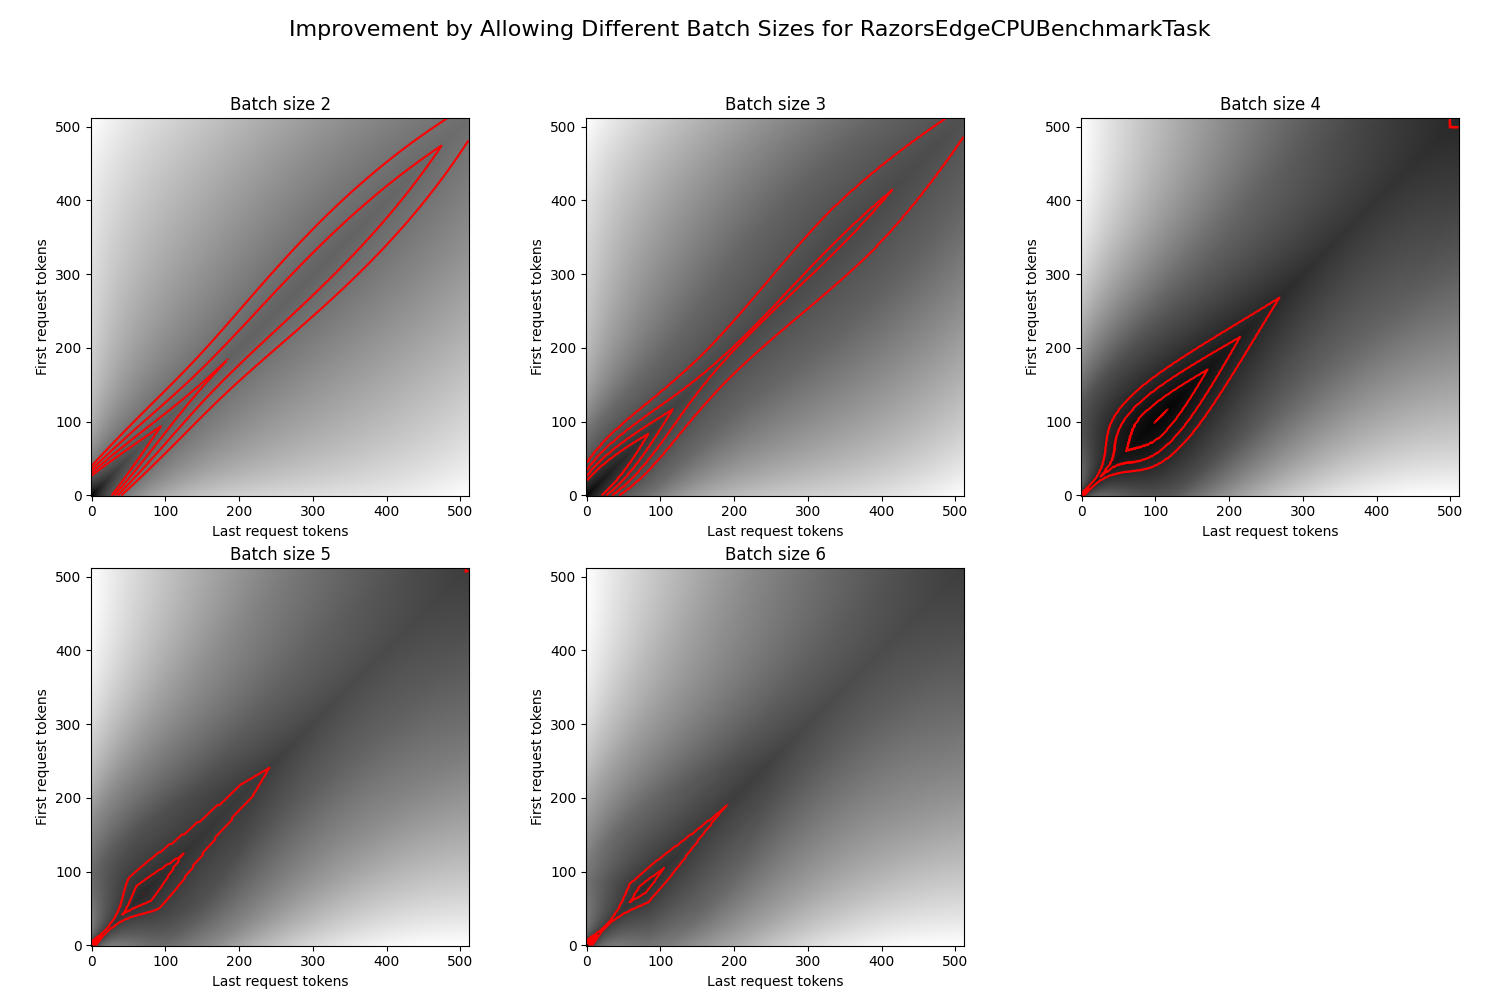
\includegraphics[width=\linewidth]{images_latex/Improvement_by_Allowing_Different_Batch_Sizes_for_RazorsEdgeCPUBenchmarkTask.png}

\hypertarget{77-summary-of-findings}{%
\subsection{Summary of Findings}\label{77-summary-of-findings}}

Across both workloads, we observe:

\begin{itemize}
\tightlist
\item
  Razor\textquotesingle s Edge outperforms simple batching strategies
\item
  Razor\textquotesingle s Edge enables performance gains even when
  simple batching strategies degrade performance relative to no batching
\item
  Input size dependent batching structure: batching efficiency exhibits
  a transition driven by memory-bound vs. compute-bound regimes.
\item
  Throughput improvement under load: Razor\textquotesingle s Edge
  increases effective throughput as concurrency grows by enabling better
  batch construction.
\end{itemize}

Together, these results demonstrate that, on the evaluated workloads and
setup, Razor\textquotesingle s Edge improves batching efficiency and
exhibits load-adaptive behavior relative to the baselines considered in
this paper.

\hypertarget{8-limitations-and-future-work}{%
\section{Limitations and Future
Work}\label{8-limitations-and-future-work}}

\begin{itemize}
\tightlist
\item
  Partitioning and candidate evaluation add CPU overhead. This may cause
  slowdowns for very small models, CPU-constrained environments, or
  large batch sizes.
\item
  Timing estimators could be created directly from model architecture
  and benchmarking basic operations.
\item
  It is unknown why FIFO sometimes shows slightly higher throughput in
  certain settings. One possible explanation is that FIFO can randomly
  select more "efficient" small, fast batches, while tail-aware policies
  (for example MINMAX) may sometimes deprioritize those batches.
\end{itemize}

Future work includes:

\begin{enumerate}
\def\labelenumi{\arabic{enumi}.}
\tightlist
\item
  Better estimators by analysis of model components
\item
  Estimator uncertainty modeling and online recalibration.
\item
  Throughput may be further improved by explicitly selecting the most
  hardware-efficient candidate batches.
\item
  Open-loop and bursty traffic evaluation with SLO-oriented metrics (for
  example throughput/latency frontier and p95/p99 miss-rate curves).
\item
  Broader baseline comparisons against additional production-oriented
  dynamic batching policies under matched hardware/software settings.
\end{enumerate}

\hypertarget{9-conclusion}{%
\section{Conclusion}\label{9-conclusion}}

Razor\textquotesingle s Edge provides a practical batching framework
that unifies throughput optimization and latency objectives for
variable-size inference workloads. Our core contribution is a systems
synthesis: DP-based contiguous partitioning on sorted requests,
production-oriented online strategy selection (\texttt{FIFO},
\texttt{MINMAX}, \texttt{GUARDED\_BATCH\_SIZE}), and practical estimator
construction for deployment. In the evaluated synthetic and real
(\texttt{BAAI/bge-m3}, \texttt{jinaai/jina-embeddings-v2-base-en})
settings with calibrated timing estimators, this combination improves
throughput and maintains favorable latency behavior relative to the
tested FIFO/fixed-cap baselines.

Validated in this paper:

\begin{itemize}
\tightlist
\item
  On the reported experiments, the proposed scheduler outperforms the
  defined baselines on throughput for the tested variable-size batched
  inference tasks.
\item
  The observed contour structure and load-scaling behavior are
  reproducible within the tested synthetic and \texttt{BAAI/bge-m3},
  \texttt{jinaai/jina-embeddings-v2-base-en} setups.
\end{itemize}

Not claimed:

\begin{itemize}
\tightlist
\item
  A universal guarantee across all serving stacks, models, and hardware.
\item
  Global optimality of the multi-group online latency ordering pass.
\end{itemize}

Accordingly, the method should be interpreted as an objective-driven,
empirically supported scheduler design for the evaluated workload class,
rather than a general theorem about all inference systems.

This manuscript emphasizes transparent release of code, estimator
artifacts, and reproducible replay analyses; expanded system-level
evaluations and broader baseline suites are a natural next step.

\hypertarget{10-funding-and-conflict-of-interest}{%
\section{Funding and Conflict of
Interest}\label{10-funding-and-conflict-of-interest}}

\begin{itemize}
\tightlist
\item
  \textbf{Funding:} None.
\item
  \textbf{Conflict of interest:} The author declares no competing
  financial or non-financial interests related to this work.
\end{itemize}

\hypertarget{11-ethical-considerations--potential-misuse}{%
\section{Ethical Considerations / Potential
Misuse}\label{11-ethical-considerations--potential-misuse}}

This work improves serving efficiency and resource allocation for
batched inference systems. In deployment, operators should monitor
service stability when these mechanisms are integrated. Efficiency gains
can also vary based on random variance at startup or request size
distribution. Latency objectives should be selected carefully based on
the application. Startup time will increase due to estimator creation,
which can degrade service in some applications.

\hypertarget{12-reproducibility-notes}{%
\section{Reproducibility Notes}\label{12-reproducibility-notes}}

Repository:
\url{https://github.com/arrmansa/Razors-Edge-batching-scheduler}. To
reproduce results (throughput, strategy comparisons, and historical RMS
transitivity checks) and figures, install the released package with
\texttt{pip\ install\ razors-edge-batching-scheduler} (or install
dependencies from \texttt{requirements.txt} for full local development),
open each notebook in \path{demos/}, and execute \textbf{Run All} from
the first cell in a clean kernel. Generated plots will be saved in
\texttt{images/}.

Seeds are set in notebooks where appropriate for deterministic or
near-deterministic sections of the experiments.

For the estimator-array replay validation and ablation in Section
7.2.1-7.2.2:

\begin{itemize}
\tightlist
\item
  generate estimator arrays with
  \path{demos/scheduler_tests/save_estimators_for_simulation.ipynb}
\item
  run
  \texttt{python\ demos/scheduler\_tests/generate\_simulation\_results.py}
\item
  inspect \texttt{simulation\ results.md} and
  \path{demos/scheduler_tests/simulation_results.json}
\item
  optional notebook walkthroughs:

  \begin{itemize}
  \tightlist
  \item
    \path{demos/scheduler_tests/simulation_strategy_tests_saturated_enhanced.ipynb}
  \item
    \path{demos/scheduler_tests/simulation_strategy_tests_saturated_ablation.ipynb}
  \end{itemize}
\end{itemize}

We keep benchmark-critical dependencies in \texttt{requirements.txt};
non-benchmark package version changes (for example notebook
tooling/plotting helpers) should not materially change measured
throughput trends.

Absolute throughput values can vary across hardware and runtime
conditions, but the contour-shape phenomenon ("razor\textquotesingle s
edge" transition between efficient and inefficient batching regions) is
expected to be present on most modern hardware and models.

All figures have source notebooks provided.

The paper text describes implemented behavior and references concrete
function names in:

\begin{itemize}
\tightlist
\item
  \path{src/razors_edge/optimal_batching.py}
\item
  \path{src/razors_edge/optimal_benchmarking.py}
\item
  \path{src/razors_edge/razors_edge_compute_task.py}
\item
  \path{src/batching_executor/base_batched_compute_task.py}
\item
  \path{src/batching_executor/process_manager.py}
\end{itemize}

\hypertarget{13-references}{%
\section{References}\label{13-references}}

{[}1{]} W. E. Smith, "Various optimizers for single-stage production,"
\emph{Naval Research Logistics Quarterly}, vol. 3, no. 1-2, pp. 59-66,
1956.

{[}2{]} U. Bagchi, Y. L. Chang, and R. S. Sullivan, "Minimizing squared
deviation of completion times about a common due date," Manag. Sci.,
vol. 33, no. 7, pp. 894--906, Jul. 1987.

{[}3{]} S. K. Gupta and T. Sen, "Minimizing a quadratic function of job
lateness on a single machine," Eng. Costs Prod. Econ., vol. 7, no. 3,
pp. 187--194, Sep. 1983.

{[}4{]} NVIDIA, "Dynamic Batcher," Triton Inference Server
Documentation.
\url{https://docs.nvidia.com/deeplearning/triton-inference-server/user-guide/docs/user_guide/batcher.html}
(accessed 2026-03-24).

{[}5{]} mixedbread-ai, "batched" (GitHub repository).
\url{https://github.com/mixedbread-ai/batched} (accessed 2026-03-24).

{[}6{]} michaelfeil, "infinity" integrations (GitHub repository).
\url{https://github.com/michaelfeil/infinity?tab=readme-ov-file\#integrations}
(accessed 2026-03-24).

{[}7{]} Hugging Face, "Pipeline batch inference" documentation.
\url{https://huggingface.co/docs/transformers/pipeline_tutorial\#batch-inference}
(accessed 2026-03-24).


\end{document}
